\documentclass[12pt,
openright, 
oneside, %
%twoside, %TCC: Se seu texto tem mais de 100 páginas, descomente esta linha e comente a anterior
a4paper,    %
%english,   %
brazil]{facom-ufu-abntex2}

\usepackage{graphicx}
\graphicspath{{figuras/}{pictures/}{images/}{./}} % where to search for the images

\newcommand{\blue}[1]{\textcolor{blue}{#1}}
\newcommand{\red}[1]{\textcolor{red}{#1}}


% ##################
% Pacotes adicionados por mim (além dos do modelo!)
% ##################

%Pacote de quotations (aspas)
\usepackage[autostyle=true]{csquotes}
% % Pacote para caixas de texto de borda colorida (usadas na exibição de código)
% \usepackage{tcolorbox}
% Pacote usado para exibição de código
\usepackage{listings}
% Pacotes para tabelas
\usepackage[table,xcdraw]{xcolor}

% ##################
% Configurando estilos de código para o pacote listings. A linguagem padrão é Python, mas pode ser modificada em cada listing com a config "language=<linguagem>,"
% Créditos para a config modificada e usada aqui: https://tex.stackexchange.com/a/83883/295210
% ##################

% Redefinindo o nome usado nos trechos de código ("Listing" -> "Algoritmo")
\renewcommand{\lstlistingname}{Algoritmo}
% Redefinindo o nome usado no título da parte de lista de listings ("List of Listings" -> "Lista de Algoritmos")
\renewcommand{\lstlistlistingname}{Lista de \lstlistingname s}

% Default fixed font does not support bold face
\DeclareFixedFont{\ttb}{T1}{txtt}{bx}{n}{12} % for bold
\DeclareFixedFont{\ttm}{T1}{txtt}{m}{n}{12}  % for normal

% Custom colors
% \usepackage{color}
\definecolor{deepblue}{rgb}{0.0, 0.0, 0.5}
\definecolor{deepred}{rgb}{0.6, 0.0, 0.0}
\definecolor{deepgreen}{rgb}{0.0, 0.5, 0.0}
\definecolor{darkergray}{rgb}{0.5, 0.5, 0.5}
% \definecolor{magenta}{rgb}{1.0.0, 0.0, 1.0}
\definecolor{linenumber}{rgb}{0.5, 0.5, 0.5}

% Code style for highlighting
\newcommand\codestyle{\lstset{
language=Python,
basicstyle=\ttm\smaller,
morekeywords={self},                  % Add keywords here
keywordstyle=\ttb\color{deepblue},
% emph={MyClass,__init__},            % Custom highlighting
% emphstyle=\ttb\color{deepred},      % Custom highlighting style
stringstyle=\color{deepgreen},
commentstyle=\color{darkergray},
% morecomment=[l][\color{magenta}]{\#}, % "Include" lines in C++
% morecomment=[l][\color{magenta}]{\# }, % "Include" lines in C++
frame=tb,                             % Any extra options here
showstringspaces=false,
% 
% Options added by me
% 
breaklines=true,
breakatwhitespace=true,
numbers=left,                         % where to put the line-numbers; possible values are (none, left, right)
numbersep=5pt,                        % how far the line-numbers are from the code
numberstyle=\tiny\color{linenumber},  % the style that is used for the line-numbers
rulecolor=\color{black},              % if not set, the frame-color may be changed on line-breaks within not-black text (e.g. comments (green here))
}}


% Code environment
\lstnewenvironment{code}[1][]
{
\codestyle
\lstset{#1}
}
{}

% Command for external code files
\newcommand\codeexternal[2][]{{
\codestyle
\lstset{inputencoding=utf8}
\lstinputlisting[#1]{#2}}}

% Command for inline code
\newcommand\codeinline[1]{{\codestyle\lstinline!#1!}}

% ##################
% Configurações gerais do pacote listings --- estas necessariamente tem que vir depois dos estilos configurados anteriormente
% ##################

% Configurando chars unicode não suportados por padrão
\lstset{literate=
  {á}{{\'a}}1 {é}{{\'e}}1 {í}{{\'i}}1 {ó}{{\'o}}1 {ú}{{\'u}}1
  {Á}{{\'A}}1 {É}{{\'E}}1 {Í}{{\'I}}1 {Ó}{{\'O}}1 {Ú}{{\'U}}1
  {à}{{\`a}}1 {è}{{\`e}}1 {ì}{{\`i}}1 {ò}{{\`o}}1 {ù}{{\`u}}1
  {À}{{\`A}}1 {È}{{\`E}}1 {Ì}{{\`I}}1 {Ò}{{\`O}}1 {Ù}{{\`U}}1
  {ä}{{\"a}}1 {ë}{{\"e}}1 {ï}{{\"i}}1 {ö}{{\"o}}1 {ü}{{\"u}}1
  {Ä}{{\"A}}1 {Ë}{{\"E}}1 {Ï}{{\"I}}1 {Ö}{{\"O}}1 {Ü}{{\"U}}1
  {â}{{\^a}}1 {ê}{{\^e}}1 {î}{{\^i}}1 {ô}{{\^o}}1 {û}{{\^u}}1
  {Â}{{\^A}}1 {Ê}{{\^E}}1 {Î}{{\^I}}1 {Ô}{{\^O}}1 {Û}{{\^U}}1
  {ã}{{\~a}}1 {ẽ}{{\~e}}1 {ĩ}{{\~i}}1 {õ}{{\~o}}1 {ũ}{{\~u}}1
  {Ã}{{\~A}}1 {Ẽ}{{\~E}}1 {Ĩ}{{\~I}}1 {Õ}{{\~O}}1 {Ũ}{{\~U}}1
  {œ}{{\oe}}1 {Œ}{{\OE}}1 {æ}{{\ae}}1 {Æ}{{\AE}}1 {ß}{{\ss}}1
  {ű}{{\H{u}}}1 {Ű}{{\H{U}}}1 {ő}{{\H{o}}}1 {Ő}{{\H{O}}}1
  {ç}{{\c c}}1 {Ç}{{\c C}}1 {ø}{{\o}}1 {Ø}{{\O}}1 {å}{{\r a}}1 {Å}{{\r A}}1
  {€}{{\euro}}1 {£}{{\pounds}}1 {«}{{\guillemotleft}}1
  {»}{{\guillemotright}}1 {ñ}{{\~n}}1 {Ñ}{{\~N}}1 {¿}{{?`}}1 {¡}{{!`}}1 
  % Novas adições feitas por mim
  {…}{{...}}1 {–}{{--}}1 {—}{{---}}1
}

% Definindo a numeração dos blocos do pacote "listings" para ser por documento, e não por capítulo
\lstset{numberbychapter=false}

% ##################

% ---
% Informações de dados para CAPA e FOLHA DE ROSTO
% ---

\autor{Vinícius Henrique Almeida Praxedes} %TCC
\data{2023, Novembro}
\orientador{Daniel Duarte Abdala} %TCC
%\coorientador{Algum?} %TCC

\titulo{Paralelização de Algoritmos Notórios de Agrupamento de Dados em GPUs NVIDIA} %TCC

\hypersetup{pdfkeywords={palavra 1}{palavra 2}{palavra 4}{palavra 4}{palavra 5}} %TCC





% * ############################################################################
% * Variáveis e macros
% * ############################################################################

\def\qntAlgrtm{dois}
\def\qntAlgrtmNaoExtenso{2}





% * ############################################################################
% * Documento
% * ############################################################################

\begin{document}
\frenchspacing

% ----------------------------------------------------------
% ELEMENTOS PRÉ-TEXTUAIS
% ----------------------------------------------------------
%\pretextual
\imprimircapa
\imprimirfolhaderosto


% ---
% Inserir folha de aprovação
% ---
%
% \includepdf{folhadeaprovacao_final.pdf} %TCC: depois de aprovado o trabalho, descomente esta linha e comente o próximo bloco para incluir scan da folha de aprovação.
%
\begin{folhadeaprovacao}

  \begin{center}
    {\ABNTEXchapterfont\large\imprimirautor}

    \vspace*{\fill}\vspace*{\fill}
    {\ABNTEXchapterfont\bfseries\Large\imprimirtitulo}
    \vspace*{\fill}
    
    \hspace{.45\textwidth}
    \begin{minipage}{.5\textwidth}
        \imprimirpreambulo
    \end{minipage}%
    \vspace*{\fill}
   \end{center}
    
   Trabalho aprovado. \imprimirlocal, 01 de novembro de 2016: %TCC:

   \assinatura{\textbf{\imprimirorientador} \\ Orientador}  
   \assinatura{\textbf{Professor}}% \\ Convidado 1} %TCC:
   \assinatura{\textbf{Professor}}% \\ Convidado 2} %TCC:
   %\assinatura{\textbf{Professor} \\ Convidado 3}
   %\assinatura{\textbf{Professor} \\ Convidado 4}
      
   \begin{center}
    \vspace*{0.5cm}
    {\large\imprimirlocal}
    \par
    {\large\imprimirdata}
    \vspace*{1cm}
  \end{center}
  
\end{folhadeaprovacao}
% ---


%%As seções dedicatória, agradecimento e epígrafe não são obrigatórias.
%%Só as mantenha se achar pertinente.

% ---
% Dedicatória
% ---
%\begin{dedicatoria}
%   \vspace*{\fill}
%   \centering
%   \noindent
%   \textit{Dedico a \lipsum[10]}  %TCC:
%   \vspace*{\fill}
%\end{dedicatoria}
% ---

% ---
% Agradecimentos
% ---
%\begin{agradecimentos}
%Agradeço a \lipsum[30]. %TCC:
%\end{agradecimentos}
% ---

% ---
% Epígrafe
% ---
%\begin{epigrafe}
%    \vspace*{\fill}
%  \begin{flushright}
%    \textit{``Alguma citação que ache conveniente? \lipsum[10]''} %TCC:
%  \end{flushright}
%\end{epigrafe}
% ---



% * ############################################################################
\begin{resumo}
% * ############################################################################

% TODO
% TODO
% ! TODO: Escrever o resumo, depois de concluir o resto do trabalho!
% TODO
% TODO

\textbf{TODO: Escrever o resumo após terminar a monografia}. Segundo a \citeonline[3.1-3.2]{NBR6028:2003}, o resumo deve ressaltar o
objetivo, o método, os resultados e as conclusões do documento. A ordem e a extensão
destes itens dependem do tipo de resumo (informativo ou indicativo) e do
tratamento que cada item recebe no documento original. O resumo deve ser
precedido da referência do documento, com exceção do resumo inserido no
próprio documento. (\ldots) As palavras-chave devem figurar logo abaixo do
resumo, antecedidas da expressão Palavras-chave:, separadas entre si por
ponto e finalizadas também por ponto.

\vspace{\onelineskip}
  
\noindent
\textbf{Palavras-chave}: Até, cinco, palavras-chave, separadas, por, vírgulas.

\end{resumo}





% * ############################################################################

% ##################
% Inserir lista de ilustrações
% ##################

\pdfbookmark[0]{\listfigurename}{lof}
\listoffigures*
\cleardoublepage



% ##################
% Inserir lista de tabelas
% ##################

\pdfbookmark[0]{\listtablename}{lot}
\listoftables*
\cleardoublepage



% ##################
% inserir lista de abreviaturas e siglas
% ##################

\begin{siglas}
  % \item[Fig.] Area of the $i^{th}$ component
  % \item[456] Isto é um número
  % \item[123] Isto é outro número
  % \item[Zézão] este é o meu nome
  \item[CPU] \textit{Central Processing Unit} --- Unidade de Processamento Central. O principal e mais importante processador num computador. CPUs modernas possuem capacidade razoável de processamento paralelo, com dezenas de núcleos
  \item[GPU] \textit{Graphics Processing Unit} --- Unidade de Processamento de Gráficos. Um coprocessador especializado para operações vetoriais, comumente usado para operações da computação gráfica, como renderização de imagens. GPUs modernas possuem capacidade altíssima de processamento paralelo, com centenas a milhares de núcleos
  \item[VRAM] \textit{Video Random Access Memory} --- Memória de Vídeo de Acesso Randômico. Um componente das GPUs que equivale à RAM das CPUs. Uma memória volátil de alta velocidade, usada para armazenamento de dados necessários às operações gráficas realizadas pela GPU
  \item[CUDA] [inserir informação]
\end{siglas}



% ##################
% Inserir lista de símbolos, se for adequado ao trabalho.
% ##################

%\begin{simbolos}
  %  \item[$ \Gamma $] Letra grega Gama
  %  \item[$ \Lambda $] Lambda
%  \item[$ \zeta $] Letra grega minúscula zeta
%  \item[$ \in $] Pertence
%\end{simbolos}

% ##################
% Inserir o sumario
% ##################

\pdfbookmark[0]{\contentsname}{toc}
\tableofcontents*
\cleardoublepage





% * ############################################################################
% * ELEMENTOS TEXTUAIS
% * ############################################################################

\textual





% * ############################################################################
\chapter{Introdução}
% * ############################################################################

A busca pelo menor tempo de execução é uma diretriz ubíqua na computação. Desde os primórdios da área buscamos algoritmos e procedimentos que, dados os mesmos parâmetros de entrada, executem a mesma tarefa na menor quantidade de tempo possível. Outros recursos como espaço de memória utilizado, eficiência energética ou uso da rede em muitos cenários são mais importantes que o tempo de execução, mas ainda assim ela continua sendo um dos mais estudados parâmetros para categorização e avaliação de algoritmos e procedimentos na computação. De fato o tempo de execução --- em ciclos, ou passos, de processamento --- é a métrica utilizada na análise de uma das maiores incógnitas da computação, o problema P versus NP.

% TODO
% TODO
% TODO: Adicionar no parágrafo acima uma citação básica sobre o problema P vs NP
% TODO
% TODO

Um grande avanço na quantidade de poder de processamento dos computadores e, portanto, diminuição do tempo de execução de algoritmos, foi a criação dos processadores multinúcleo, permitindo a paralelização de processos. A habilidade de poder executar duas ou mais ações simultaneamente possibilitou muitos ganhos palpáveis na velocidade de execução de algoritmos e procedimentos, porém introduziu uma necessidade de mudança na forma de se pensar em resoluções de problemas computacionalmente: paralelizar um algoritmo serial (não-paralelo) não é uma tarefa trivial, e requer cuidados especiais com concorrência no acesso a recursos da máquina, interdependência de dados e cálculos, sincronização, entre outros dilemas.

Um dos componentes que mais utilizam da paralelização num computador moderno são as GPUs --- unidades de processamento gráfico, ou placas de vídeo --- que são basicamente processadores especializados em operações vetoriais, altamente paralelizadas, usualmente utilizadas para computação gráfica, e com sua própria memória dedicada, a VRAM. Enquanto processadores de uso geral, CPUs, costumam ter no máximo dezenas de núcleos para processamento paralelo, GPUs possuem dezenas, milhares, de núcleos para operações vetoriais.

No entanto, cada vez mais está sendo descoberto e aproveitado o potencial de uso das GPUs em atividades não apenas voltadas para renderização, interfaces e outras operações gráficas, mas sim para a computação de propósito geral. Diversos algoritmos modernos e antigos beneficiam-se imensamente do poder de alta paralelização proporcionado pelas GPUs, e com ferramentas como a biblioteca e linguagem CUDA criada pela NVIDIA, está cada vez mais fácil implementar o uso de placas de vídeo em conjunto com processadores convencionais nos mais variados algoritmos.

Nem todo algoritmo pode ser paralelizado, no entanto. Existem procedimentos e algoritmos que são inerentemente seriais (também chamados de sequenciais), como o cálculo do $n$-ésimo número da sequência de \textit{Fibonacci}, que requer que dois números prévios da sequência tenham sido calculados para obtermos o atual --- salvo, é claro, alguma descoberta teórica matemática do comportamento da sequência que nos permitisse uma nova maneira de calcular o $n$-ésimo elemento sem essa necessidade.

É importante entender também que nenhum algoritmo é paralelizável por completo. Sempre existirão partes de algoritmos que necessariametne devem ser executadas serialmente para seu funcionamento correto. Há um limite teórico de ganho máximo que pode ser obtido ao se paralelizar um algoritmo qualquer. Esse limite é definido pela Lei de Amdahl \cite{Amdahl-Law}: $\frac{1}{1-p}$, onde $p$ é a razão entre tempo de execução gasto rodando código paralelizável e tempo de execução gasto no total.

E é a paralelização de uma classe de algoritmos em particular que é o foco desta pesquisa: os algoritmos de agrupamento de dados, também chamados de clusterização de dados, ou de \textit{clustering}. Tais algoritmos, de forma sucinta, agrupam objetos de maneira que os objetos no mesmo grupo, ou \textit{cluster}, sejam mais parecidos entre si, de acordo com alguma métrica, do que com objetos de outros grupos. A análise de clusters é essencial em diversas áreas da computação e estatística, como mineração de dados, aprendizado de máquina, compressão de dados, entre outras.

A hipótese principal deste trabalho é a de que algoritmos de clustering, em geral, são altamente paralelizáveis e apresentam um ganho considerável de desempenho (menor tempo de execução) quando implementados para utilizar o poder de paralelismo vetorial de placas de vídeo NVIDIA, através da linguagem CUDA \cite{CUDAZone}. Mais que isso, através de uma análise sistemática de estudos prévios e implementações de tais algoritmos em CUDA, visa-se generalizar o processo de paralelização destes. Isto é, identificar quais partes são necessariamente seriais, quais são paralelizáveis, e que sequência de passos gerais deve ser seguida para se conseguir paralelizar com sucesso um algoritmo de clustering qualquer e obter ganhos significativos de desempenho.

% TODO
% TODO
% TODO: Revisar todos acronismos (definir as siglas todas no primeiro uso, e apenas no primeiro uso)
% TODO
% TODO

% TODO
% TODO
% ! TODO: Tenho que substituir essas referências abaixo por referências de versões seriais de cada algoritmo. Usar as referências das versões aceleradas em GPUs mais adiante, ao invés de aqui parece fazer bem mais sentido
% TODO
% TODO

O foco de pesquisa é o notório algoritmo de agrupamento \textit{k-means} \cite{GPU-accelerated-K-Means}. Implementações e estudos realizados sobre ele foram analisados, e uma implementação paralela em GPU teve seu desempenho comparado com a serial em CPU.

% * Texto antigo do parágrafo acima:
% O foco de pesquisa são \qntAlgrtm{} algoritmos de agrupamento especialmente notórios: o \textit{k-means} \cite{GPU-accelerated-K-Means} e o \textit{Agrupamento Hierárquico}. Implementações e estudos realizados sobre estes foram analisados, e implementações paralelas em GPU tiveram seu desempenho comparado com as seriais em CPU.


% * Texto ainda mais antigo do parágrafo acima:
% , \textit{DBSCAN} \cite{G-DBSCAN}, ou \textit{Clusterização Espacial Baseada em Densidade de Aplicações com Ruído}, e \textit{Random Forests} --- que mesmo não sendo exclusivamente um algoritmo de clusterização, pode ser utilizado justamente para tal.



% * ####################################

\section{Objetivos}



% * ####################################

\subsection{Objetivo Geral}

Este trabalho tem como objetivo principal testar a validez de sua hipótese (discutida mais à fundo na seção 1.2) de que algoritmos de clusterização são intrinsecamente paralelizáveis, e que o ganho de velocidade ao serem paralelizados é altamente significativo.

Além disso, deseja-se compilar aqui um vasto conhecimento de como paralelizar esses algoritmos em geral, analisando principalmente os \qntAlgrtm{} aqui estudados a fundo (k-means e agrupamento hierárquico) e usando este aprendizado para criar um passo-a-passo genérico de como realizar tal modificação de código em um algoritmo de agrupamento qualquer.



% * ####################################

\subsection{Objetivos Específicos}

Para atingir o objetivo geral, é necessário completar diversos objetivos menores, ou \textit{milestones}, antes, criando um caminho de pesquisa que foi seguido --- não necessariamente na ordem apresentada. São estes:

\begin{itemize}
  \item Pesquisar extensamente a bibliografia da área, realizando assim um levantamento do estado da arte de algoritmos paralelos de agrupamento;
  
  \item Estudar implementações já realizadas dos \qntAlgrtm{} algoritmos aqui estudados, a fim de adquirir conhecimento de como a paralelização em CUDA deve ser realizada;
  
  \item Paralelizar um algoritmo de clustering \enquote{novo}, isto é, nunca antes paralelizado e exibido em trabalho científico, a fim de solidificar o conhecimento e prática de programação em CUDA. Foi escolhido o algoritmo de Agrupamento Hierárquico para tal;
  
  \item Quantificar o ganho de desempenho das implementações paralelas, realizando diversos experimentos de \textit{speedup}, usando diversos datasets de tamanhos e dimensionalidades variadas;
  
  \item Comparar o código serial (sem paralelização) com o código paralelo dos \qntAlgrtm{} algoritmos analisados, extraindo assim um conhecimento de como paralelizar um algoritmo de clusterização genérico;
\end{itemize}



% * ####################################

\section{Hipótese}

A hipótese que esta pesquisa procura testar é a de que algoritmos de clusterização em geral são inerentemente vetoriais e, consequentemente, se beneficiariam significativamente de arquiteturas de processamento vetoriais, como uma unidade de processamento gráfico, ou GPU.

Um problema ser vetorial diz respeito ao escopo de tipos de dados relevantes ao problema. Grande parte dos problemas da computação são escalares, o que significa que eles lidam com dados unitários, como por exemplo \textit{integers} ou \textit{floats}, um de cada vez. Já um problema vetorial lida com dados que são conjuntos unidimensionais, chamados vetores, que são formados por vários itens unitários de dados agrupados.

Um algoritmo que tente resolver um problema vetorial terá desempenho maior quando executado num processador vetorial, isto é, um processador que possui um conjunto de instruções capaz de manipular vetores. Apesar de um algoritmo de um problema vetorial ainda puder ser implementado e executado com sucesso num processador escalar, o desempenho será menor pois os dados vetoriais do problema terão que ter seus elementos processados um a um pelo processador, já que ele não trabalha com vetores propriamente ditos em seu conjunto de instruções.

Grande parte do ganho de desempenho supracitado vem do paralelismo proporcionado pelos processadores vetoriais, como GPUs, ao manipular conjuntos maiores de dados de uma só vez, e em vários núcleos simultaneamente. A natureza vetorial da GPU permite economizar traduções de endereço de memória e operações de obtenção (\textit{fetch}) e decodificação (\textit{decode}) de instruções, se comparado com o processamento escalar de uma CPU, pelo fato de se necessitar, na GPU, um número muito menor de instruções e endereços de memória quando os dados estão agrupados em vetores, que podem ser manipulados e usados em operações como se fossem, cada um, apenas um item de dados.

Este trabalho, então, visa demonstrar que algoritmos de agrupamento de dados, em geral, são intrinsecamente vetoriais. Isto é, qualquer algoritmo de clustering concebível será de natureza vetorial, pois estes analisam dados e tentam agrupá-los de acordo com algum grau de semelhança entre eles, análise esta que pode ser feita usando conjuntos dos itens de dados (vetores), ao invés de individualmente, mesmo que o \textit{dataset} inicial possua apenas dados de natureza escalar. Logo, qualquer algoritmo de agrupamento teria uma parcela do seu código que seria paralelizável e, assim, ganhariam desempenho significativo com uma execução numa GPU. Mais que isso, a parcela de tempo de execução do algoritmo gasta rodando código paralelo cresceria de acordo com o tamanho do conjunto de dados sendo analisado, garantindo ganhos ainda maiores.



% * ####################################

\section{Justificativa}

A pesquisa feita aqui pode ser de grande utilidade para a área da computação e ciência de dados, além de impulsionar a implementação de mais algoritmos paralelos de agrupamento de dados.

Com a compilação de conhecimento realizada aqui a intenção é facilitar pesquisas posteriores na área de paralelização de algoritmos de agrupamento e motivar com os experimentos de ganho de desempenho novas implementações paralelas de outros algoritmos desta classe, ilustrando o quão importante é o uso de processadores vetoriais como GPUs para tornar o uso de algumas destas abordagens de agrupamento realmente práticas.

Além disso, a apresentação nesse estudo de um procedimento genérico para paralelizar qualquer algoritmo de agrupamento será de extrema utilidade para qualquer desenvolvedor ou pesquisador que desejar implementar uma versão acelerada em GPU de um algoritmo do tipo, mesmo este sendo totalmente novo. No mínimo, a pesquisa servirá de ponto de partida para o entendimento e aprendizado de como realizar tal modificação no código do algoritmo, e renderá uma implementação real que serve de base para estudos e otimizações, até se obter eventualmente uma implementação digna para uso prático.





% * ############################################################################
\chapter{Fundamentação Teórica}
% * ############################################################################

Para compreender a pesquisa científica aqui realizada, é necessário primeiro entender o que são algoritmos de agrupamento, tanto de maneira geral quanto específica, explorando os fundamentos e funcionamento dos \qntAlgrtm{} algoritmos pesquisados. Veremos que a complexidade de tempo desses algoritmos tendem a ser inconvenientemente altas ($O(n\cdot\log{n})$, $O(n^2)$ ou até $O(n^3)$ sendo complexidades comuns) e por isso qualquer ganho de velocidade significativo obtido será de imensa relevância para a usabilidade prática do algoritmo.

Também é imprescindível explorar o funcionamento dos processadores vetoriais --- sendo as \textit{Unidades de Processamento Gráfico} (GPUs) o principal exemplo destes e exatamente no qual essa pesquisa irá focar --- e entender por que usá-los para paralelizar algoritmos de agrupamento proporcionará, em tese, um ganho de velocidade expressivo na execução destes, abrandando o peso de suas complexidades de tempo. Além de tudo isso, será apresentada brevemente a arquitetura utilizada para paralelizar os algoritmos estudados: a plataforma e modelo de programação CUDA, da NVIDIA, que permitirá extrair o poder de paralelização das placas de vídeo NVIDIA além de bibliotecas como a \textit{Numba}, que permite a programação vetorial facilitada na linguagem Python.

% TODO
% TODO
% ? TODO: Adicionar citação a respeito da biblioteca Numba aqui? Ou deixar pra fazer isso apenas ao aprofundarmos nela um pouco, mais adiante?
% SIM
% TODO
% TODO



% * ####################################

\section{Agrupamento de dados}

O agrupamento de dados, também chamado de clusterização de dados (data clustering, em inglês), é a tarefa de agrupar um conjunto de elementos de modo que cada elemento de um grupo se \enquote{pareça} mais com outros elementos do grupo (\textit{cluster}) que pertence do que com elementos dos grupos que não pertencem, dado algum significado bem definido de semelhança entre os dados. É um processo muito comum e virtualmente imprescindível nas áreas de mineração de dados, análise estatística, análise de imagem, aprendizado de máquina, reconhecimento de padrões, e muitas outras.

O significado de um cluster não pode ser bem definido e vai depender do conjunto de dados a ser analisado e a forma que os resultados obtidos serão utilizados --- de fato, esse é o principal motivo pelo qual tantos algoritmos diferentes de agrupamento existem \cite{SoManyClustAlg}. O fator comum na maioria das definições propostas é que um cluster é um conjunto de \textit{datapoints} --- pontos, ou objetos de dados ou até mesmo instâncias. Esses objetos são representados num espaço geométrico com o número de dimensões iguais ao número de variáveis necessárias para descrever cada datapoint, e os algoritmos de agrupamento tentam criar grupos nesse espaço que agrupem os objetos de uma maneira significativa, ou útil, para o estudo sendo feito e a definição de \enquote{grupo} sendo utilizada.

% TODO
% TODO
% TODO adicionar citações, figuras de agrupamento de dados
% TODO
% TODO

Diversos modelos de grupo podem ser usados para definir o que é um grupo: \textbf{modelos de centroide}, onde cada grupo possui um centro e cada datapoint pertencerá ao grupo com centro mais próximo dele, dada uma definição de distância no espaço geométrico dos dados; \textbf{modelos de densidade}, que definem grupos como regiões densas e conexas no espaço, contrastando com regiões menos densas que separam os grupos; \textbf{modelos de conectividade}, que constroem grupos a partir de conexões de datapoints definidas por um limiar de distância; \textbf{modelos de distribuição}, que utilizam de distribuições estatísticas, como a distribuição normal ou exponencial, para modelar o agrupamento dos datapoints; entre dezenas de outros modelos. Entender o modelo de grupo utilizado é essencial para compreender um algoritmo de agrupamento e as diferenças entre a multitude destes.

O resultado, ou saída, de um algoritmo de agrupamento é comumente um rotulamento dos datapoints passados na entrada, o que indicará a divisão em grupos feita por ele. Classificações podem ser feitas quanto à natureza do agrupamento obtido pelos algoritmos: \textbf{\textit{hard clustering}}, onde cada objeto pertence ou não a um grupo; \textbf{\textit{fuzzy clustering}}, onde cada objeto pertence uma certa porcentagem a cada grupo, o que pode representar, por exemplo, a chance do objeto pertencer àquele grupo, ou até o grau de semelhança do datapoint comparado aos outros datapoints de cada grupo \cite{FuzzyClusteringSurvey}. E subclassificações ainda mais granulares podem ser definidas, como: \textbf{clusterização de particionamento estrito}, onde cada objeto pertence a exatamente um cluster; \textbf{clusterização de particionamento estrito com \textit{outliers}}, onde objetos pertencem a exatamente um cluster, ou nenhum cluster, assim sendo considerados \textit{outliers}, entre outras classificações.

Os algoritmos de agrupamento são essenciais na análise de dados, permitindo a identificação de padrões e estruturas em conjuntos de dados não rotulados. Eles pertencem à categoria de \textbf{algoritmos de aprendizado não supervisionado} e são amplamente utilizados em diversas áreas da computação, matemática, economia, estatística, dentre outras. A paralelização desses algoritmos visa melhorar a eficiência computacional, permitindo o processamento mais rápido de grandes volumes de dados.



% * ####################################

\section{Programação Vetorial}

% % ? ################
% % ? Planning writing
% % ? ################

% [Escrever uma sub-seção sobre Programação Vetorial]

% \begin{itemize}
  %   \item Tópico histórico, de onde ela vem, pra que ela serve
  %   \item Processadores que dão suporte pra operações vetoriais (hoje em dia, basicamente apenas GPUs. APUs tbm?)
  %   \item História da NVIDIA criando o CUDA
%   \item Mudança de paradigma em relação à programação serial: escalar -> vetorial
% \end{itemize}

A programação vetorial é uma abordagem computacional que visa aproveitar ao máximo o potencial de processamento de unidades de processamento que suportam operações vetoriais. Essa abordagem permite realizar operações em conjuntos de dados (vetores) de uma só vez, em vez de processar individualmente cada elemento do vetor. Isso resulta em um aumento significativo no desempenho computacional, especialmente em algoritmos que manipulam grandes volumes de dados.



\subsection{História}

A história da programação vetorial é intrinsecamente ligada ao avanço da computação e à necessidade de lidar com conjuntos massivos de dados de maneira eficiente. O conceito de processamento vetorial remonta ao desenvolvimento dos primeiros supercomputadores e ao surgimento das primeiras GPUs, com destaque para a evolução da arquitetura das GPUs NVIDIA.

A ideia por trás da programação vetorial é aproveitar ao máximo o poder de processamento dos processadores, executando uma mesma instrução em múltiplos conjuntos de dados simultaneamente. Isso é especialmente útil em tarefas que envolvem operações repetitivas sobre grandes vetores ou matrizes de dados, como aquelas encontradas em algoritmos de processamento de imagem, simulações físicas e, mais recentemente, em algoritmos de agrupamento de dados.

Ao longo do tempo, a programação vetorial evoluiu significativamente, impulsionada pelo avanço das arquiteturas de processadores e pela demanda por computação paralela cada vez mais poderosa. Um dos marcos importantes nessa evolução foi a introdução do tipo de processamento SIMD (Single Instruction, Multiple Data) nos supercomputadores na década de 1970 (FLYNN, 1972). Essa abordagem permitiu que uma única instrução fosse executada em múltiplos dados simultaneamente, proporcionando um aumento significativo no desempenho computacional para uma ampla gama de aplicações.

Com o surgimento das GPUs, inicialmente desenvolvidas para renderização gráfica em jogos e aplicações de multimídia, surgiu uma nova oportunidade para a programação vetorial. As GPUs são compostas por centenas ou até milhares de núcleos de processamento, o que as torna altamente paralelizáveis e adequadas para executar operações vetoriais em larga escala. Isso possibilitou a utilização das GPUs não apenas para gráficos, mas também para tarefas de computação de propósito geral (área chamada também de \textit{GPGPU}), incluindo processamento de grandes conjuntos de dados e algoritmos de aprendizado de máquina.

Um exemplo emblemático da aplicação da programação vetorial em GPUs NVIDIA é o algoritmo de agrupamento de dados conhecido como k-means. O k-means é amplamente utilizado em análise de dados e mineração de dados para agrupar pontos de dados em clusters com base em características semelhantes. A paralelização deste algoritmo em GPUs NVIDIA pode resultar em um significativo aumento de desempenho, permitindo o processamento rápido de grandes conjuntos de dados (Shane, 2012).

Em suma, a programação vetorial desempenha um papel fundamental no avanço da computação paralela e no desenvolvimento de algoritmos eficientes para lidar com conjuntos massivos de dados. Com a contínua evolução da arquitetura de processadores e o aumento da demanda por computação paralela, é esperado que a programação vetorial continue a desempenhar um papel crucial no desenvolvimento de soluções computacionais rápidas e escaláveis para uma variedade de aplicações, como processamento de sinais, computação gráfica, simulações físicas, aprendizado de máquina e muito mais. Ela permite acelerar algoritmos complexos, reduzindo o tempo de execução e aumentando a eficiência computacional.

% Fontes (organizar no .bib posteriormente) e candidatos a fontes da sub-seção acima
% FLYNN, Michael J. Some computer organizations and their effectiveness. IEEE transactions on computers, v. 100, n. 9, p. 948-960, 1972. - https://andreprzybysz.com/2023/04/19/classificacao-de-flynn-para-categorizar-as-arquiteturas-de-processadores/

% https://www.ufpe.br/documents/39830/745800/17_GiorgiaMattos/c2c5feb6-6e54-461b-b761-7e22900857d8

% (Shane, 2012) ?



\subsection{Processadores Vetoriais}
\label{ssc:vetorial}

É importante entender que nem todo processador oferece suporte para operações vetoriais, ou as oferecem com níveis de paralelismo inferiores a outros tipos de processadores mais especializados. Essas operações são essenciais para o desenvolvimento de algoritmos eficientes em uma variedade de aplicações computacionais. Examina-se aqui a arquitetura e as capacidades de diversos tipos de processadores, destacando sua importância na aceleração de operações paralelas e no aumento da eficiência computacional.

Os \textbf{processadores} com suporte de processamento paralelo \textbf{SIMD} desempenham um papel crucial na execução de operações vetoriais, permitindo a aplicação de uma única instrução em múltiplos conjuntos de dados simultaneamente. Esse tipo de processamento paralelo foi o foco de extensões como as SSE (\textit{Streaming SIMD Extensions}), que permitiram um grande aumento de performance na execução de aplicações como processamento de sinal digital e processamento gráfico. Essas extensões são encontradas na gigantesca maioria das CPUs x86 atuais, a família de arquiteturas de processadores mais usada até hoje em computadores pessoais.

Os \textbf{processadores VLIW} (\textit{Very Long Instruction Word}) são definidos pela sua capacidade de executar múltiplas operações em paralelo por meio de instruções muito longas. Destaca-se sua presença em sistemas embarcados e a eficiência proporcionada pela execução simultânea de operações vetoriais, especialmente em aplicações de processamento de sinal e comunicações digitais. Arquiteturas deste tipo já foram amplamente utilizadas em GPUs, porém houve uma mudança para arquiteturas RISC (\textit{Reduced Instruction Set Computer}), mais simples, para acelerar também a execução de tarefas não-gráficas.

As \textbf{Unidades de Processamento Gráfico} (\textit{Graphical Processing Units}), ou GPUs, são processadores especializados em operações úteis para aplicações gráficas, como cálculos geométricos para renderização 3D, mapeamento de texturas, rotação ou translação de vértices, aplicação de \textit{shaders}, aceleração de decodificação de vídeo, entre muitas outras. Tais operações na grande maioria dos casos envolvem vetores ou matrizes sendo manipuladas, com cálculos sendo aplicados a todos seus elementos. Logo, para lidar eficientemente com essas operações, esses processadores possuem uma unidade de memória dedicada (VRAM, \textit{Video RAM}) e empregam milhares de núcleos para processamento paralelo.

As GPUs, sendo processadores intrinsecamente vetoriais, são o foco deste trabalho. Com o advento de ferramentas como a arquitetura CUDA para GPUs produzidas pela NVIDIA, se tornou cada vez mais fácil utilizar esses processadores para aplicações gerais, não apenas gráficas, como é o caso estudado aqui, de se utilizar tais processadores para acelerar algoritmos de agrupamento de dados.

Há também os \textbf{processadores DSP} (\textit{Digital Signal Processors}), caracterizados pela sua eficiência na execução de operações vetoriais em tempo real, com foco em aplicações de processamento de sinais digitais. Possuem alta capacidade de lidar com operações complexas de forma rápida e precisa, contribuindo para o desenvolvimento de sistemas de comunicação e multimídia.

Este segmento aborda uma variedade de processadores especializados em diferentes domínios, como processamento de imagens, áudio e vídeo. Destaca-se sua arquitetura --- muitas vezes utilizando um conjunto de instruções VLIW --- otimizada para operações específicas do domínio e a incorporação de operações vetoriais para melhorar o desempenho em aplicações especializadas.

As \textbf{TPUs} (\textit{Tensor Processing Units}) são unidades de processamento especializadas desenvolvidas pela Google para otimizar operações relacionadas a tensores --- abstrações geométricas que podem ser representadas como vetores multidimensionais, usadas largamente em algoritmos de aprendizado de máquina e servindo de base para a biblioteca \textbf{TensorFlow}, também desenvolvida pela Google. Esses processadores Possuem uma arquitetura voltada para operações matriciais e vetoriais, e contribuem para acelerar o treinamento e a inferência de modelos de inteligência artificial.

O estudo dos processadores que suportam operações vetoriais revela a diversidade de arquiteturas e tecnologias disponíveis para acelerar o processamento paralelo em uma variedade de domínios. Esses processadores desempenham um papel crucial no desenvolvimento de algoritmos eficientes e na melhoria do desempenho computacional em aplicações exigentes. O contínuo avanço dessas tecnologias promete impulsionar ainda mais a inovação na computação e expandir os limites do que é possível realizar com eficiência computacional.



\subsection{Mudança do Paradigma Serial para o Vetorial}

A mudança de paradigma da programação serial para a programação vetorial representa uma verdadeira revolução na eficiência computacional. Antes da adoção generalizada da programação vetorial, os algoritmos eram projetados para serem executados de maneira sequencial, o que limitava significativamente o desempenho e a capacidade de lidar com conjuntos de dados massivos. Com a programação vetorial, no entanto, os desenvolvedores podem realizar operações em grandes conjuntos de dados de forma paralela, aproveitando ao máximo o poder de processamento disponível \cite{hennessy2011}.

Um exemplo clássico da mudança de paradigma da programação serial para a programação vetorial pode ser observado na computação gráfica. Antes da adoção da programação vetorial, o processo de renderização de imagens em 3D exigia a aplicação de algoritmos sequenciais para calcular cada pixel individualmente. Com a introdução da programação vetorial através do CUDA, por exemplo, os desenvolvedores podem aproveitar a capacidade das GPUs para realizar cálculos em paralelo, acelerando significativamente o processo de renderização e permitindo a criação de gráficos mais realistas e complexos em tempo real.

Outro exemplo impactante da mudança é encontrado no campo do aprendizado de máquina. Antes da adoção da programação vetorial, os algoritmos de aprendizado de máquina muitas vezes enfrentavam limitações de desempenho devido à necessidade de processar grandes conjuntos de dados de forma sequencial. Com a programação vetorial e o uso de frameworks como TensorFlow e PyTorch, os desenvolvedores podem aproveitar o paralelismo das GPUs para treinar modelos complexos em um tempo significativamente menor, abrindo novas possibilidades para aplicações de inteligência artificial em tempo real e análise de big data.

Embora a programação vetorial ofereça inúmeras vantagens em termos de eficiência computacional e desempenho, ela também apresenta desafios significativos. A otimização de algoritmos para aproveitar ao máximo o paralelismo disponível e lidar com questões de sincronização e acesso concorrente aos recursos do sistema tornou-se uma prioridade para os desenvolvedores. No entanto, esses desafios também representam oportunidades de inovação e avanço na área de computação paralela, incentivando o desenvolvimento de técnicas e ferramentas cada vez mais sofisticadas para maximizar o potencial da programação vetorial.

No contexto deste trabalho, serão abordadas técnicas avançadas de agrupamento de dados, incluindo o algoritmo \textit{k-means} e o \textit{Hierarchical Clustering}. A aplicação dessas técnicas em um ambiente de programação vetorial, como o CUDA, promete explorar todo o potencial de processamento paralelo das GPUs NVIDIA para acelerar significativamente a análise e o agrupamento de grandes conjuntos de dados. Ao incorporar essas técnicas em um contexto de programação vetorial, busca-se não apenas demonstrar a eficácia das abordagens de agrupamento de dados, mas também destacar o papel crucial da programação vetorial no desenvolvimento de soluções computacionais eficientes e escaláveis para problemas complexos de análise de dados.



% * ####################################

\section{NVIDIA CUDA}
\label{sec:cuda}

O CUDA (\textit{Compute Unified Device Architecture}) é uma API que permite a utilização de uma placa de vídeo com chiptset da NVIDIA para fins de computação de uso geral (\textit{GPGPU}), permitindo o acesso ao conjunto de instruções da placa e a utilização de seus diversos núcleos de processamento para a computação paralela. Foi projetada para trabalhar com linguagens de programação como \textit{Fortran}, \textit{C} e \textit{C++} e possibilita, de dentro da sintaxe delas, o acesso à memória dedicada da placa (VRAM), memória cache, o gerenciamento dos núcleos e \textit{threads} --- seu formato e quantidade ---, o escalonamento de tarefas para a CPU e GPU, bem como a transferência de dados de um para o outro.

Embora a computação de propósito geral com GPUs fosse possível antes do lançamento de APIs como CUDA, usando outras APIs mais antigas como \textit{OpenGL} ou \textit{DirectX}, o desenvolvimento era bem dificultado, necessitando a conversão de instruções de código serial e escalar para instruções de código paralelo e vetorial, basicamente obrigando desenvolvedores a \enquote{traduzir} as aplicações em análogos gráficos para serem processados como texturas ou shaders na GPU, para depois ter os resultados convertidos de volta para um formato de dados menos abstrato. O CUDA facilitou imensamente esse processo permitindo o uso do poder da GPU sem a necessidade de utilização de técnicas e APIs específicas para operações gráficas.

% * ##########################

\subsection{História}
\label{ssc:históriaCUDA}

Na virada do século, quando percebeu que desenvolvedores viam potencial nas GPUs para além do processamento gráfico, a NVIDIA começou a explorar sua capacidade para tarefas de propósito geral. Com o aumento da demanda por poder computacional e a necessidade de lidar com conjuntos massivos de dados em aplicações não relacionadas a gráficos, surgiu a ideia de utilizar as GPUs para computação paralela. Assim, em 2006, a NVIDIA lançou o CUDA como parte da arquitetura \textit{Tesla}, usada primeiro na série \textit{G80} de GPUs, marcando o início de uma nova era na computação paralela.

O lançamento do CUDA permitiu que os desenvolvedores aproveitassem o poder de processamento massivo das GPUs para uma ampla gama de aplicações computacionais \cite{cudaByExampleSanders2010}. Ao fornecer uma plataforma de programação acessível e eficiente, o CUDA abriu as portas para a aceleração de algoritmos complexos em áreas como aprendizado de máquina, simulação científica, processamento de imagens e muito mais.

Desde então, o CUDA tem passado por várias iterações e atualizações, incorporando novas tecnologias e recursos para tornar a programação em GPUs mais acessível e eficiente. Uma das principais inovações foi a introdução da arquitetura Fermi em 2010, que trouxe melhorias significativas na eficiência energética e na capacidade de processamento das GPUs NVIDIA. Com a Fermi, o CUDA ganhou suporte para novos recursos, como cálculos de precisão dupla de ponto flutuante, o que o tornou ainda mais adequado para aplicações científicas e de computação de alta precisão.

Além disso, o lançamento da arquitetura Kepler em 2012 marcou outro marco importante para o CUDA. Trouxe consideráveis melhorias na eficiência de computação e na capacidade de execução de instruções paralelas, permitindo o desenvolvimento de algoritmos mais complexos e a execução de tarefas de computação intensiva com maior eficiência.

Ao longo dos anos, o ecossistema em torno do CUDA cresceu significativamente, com uma vasta gama de ferramentas, bibliotecas e frameworks disponíveis para desenvolvedores. O lançamento do CUDA Toolkit proporcionou aos desenvolvedores um conjunto abrangente de ferramentas para desenvolver, otimizar e depurar aplicativos CUDA. Além disso, bibliotecas como cuDNN (\textit{CUDA Deep Neural Network Library}) e cuBLAS (\textit{CUDA Basic Linear Algebra Subprograms}) tornaram-se fundamentais para o desenvolvimento de aplicativos de aprendizado de máquina e processamento de dados em larga escala.

Outro aspecto importante do ecossistema CUDA é a comunidade de desenvolvedores, que continua a crescer e contribuir com uma variedade de projetos e recursos. Plataformas como o NVIDIA Developer Forums e eventos como a Conferência de Desenvolvedores NVIDIA (\textit{NVIDIA GPU Technology Conference}) desempenham um papel crucial na promoção da colaboração e na troca de conhecimentos entre os desenvolvedores CUDA em todo o mundo.

O CUDA encontrou aplicação em uma ampla variedade de setores, incluindo ciências, engenharia, medicina, finanças e entretenimento. Empresas e instituições de pesquisa em todo o mundo têm utilizado o CUDA para acelerar suas pesquisas e desenvolver soluções inovadoras para problemas complexos.

Por exemplo, na área da medicina, o CUDA é usado para acelerar simulações de dinâmica molecular e processamento de imagens médicas. No setor financeiro, ele é utilizado para análise de dados em tempo real, modelagem financeira avançada, além de possibilitar diversas implementações na área das criptomoedas e \textit{blockchains}. Na indústria de entretenimento, o CUDA é fundamental para a renderização de gráficos em filmes, jogos e animações em 3D.

Esses exemplos ilustram o impacto significativo que o CUDA teve em uma variedade de domínios, demonstrando seu papel como uma plataforma essencial para a computação paralela e o desenvolvimento de soluções de alto desempenho em todo o mundo.

% * ##########################

\subsection{Exemplo de Implementação CUDA}
\label{ssc:implementaçãoCUDA}

Para exemplificar bem o processo de paralelização de um algoritmo utilizando CUDA, é apresentada aqui uma implementação simples, na linguagem C++, de um programa que soma dois vetores unidimensionais com mais de 250 milhões de elementos cada, do tipo ponto flutuante de precisão simples (\textit{float}). Esse algoritmo então é paralelizado utilizando a API CUDA para rodá-lo em uma GPU.

Note que os dois grandes vetores inicializados ocupam cerca de 2 GB de memória no total. É importante que a máquina onde o algoritmo é executado possua essa quantidade de memória RAM disponível, assim como de VRAM na GPU. Mais detalhes sobre a máquina utilizada para testes no Capítulo \ref{sec:máquinaUtilizada}.

As implementações, assim como suas explicações contidas nesse capítulo, foram adaptadas de tutoriais disponibilizados no site \textit{NVIDIA Developer} \cite{CUDAanEvenEasierIntro}.

Os códigos de programas CUDA são salvos como arquivos com a extensão \textit{.cu}, e compilados utilizando a ferramenta \textit{nvcc}, disponível através do CUDA Toolkit \cite{CUDAtoolkit}. Existe também uma ferramenta que permite a administração, benchmark e monitoramento facilitados de programas CUDA, o \textit{Nsight Systems} disponível em \cite{NVIDIAnsightSystems}. Usando seu comando \textit{nsys nvprof} para rodar um executável CUDA, é possível realizar testes automatizados de velocidade.

O Algoritmo \ref{code:addArrayCPU.cpp} abaixo contém o programa supracitado, que soma os dois vetores, salvando no lugar dos valores do segundo vetor a soma dos valores respectivos de ambos.

\codeexternal[
  language=C++,
  % firstline=42,
  % lastline=,
  label=code:addArrayCPU.cpp,
  caption={Implementação serial de soma de vetores em C++},
]{code-snippets/addArrayCPU.cpp}

O código é bem auto-explicativo com comentários incluídos em diversas linhas. Um trecho notável é o contido nas linhas 25--28, que confere o resultado da soma para encontrar o maior erro --- definido pelo valor absoluto da subtração entre o valor encontrado no vetor e o valor esperado. Assim é possível perceber qualquer imprecisão que possa ser introduzida ao se modificar o algoritmo.

Rodando o programa e medindo o tempo de execução da função \textit{add}, é encontrado que o tempo médio entre cem execuções consecutivas é de cerca de \textbf{308 milissegundos} e o erro máximo é zero.

% ? Realmente vale a pena mostrar essa versão coitada que nem paralela na verdade é? Acho que não…

% \codeexternal[
%   language=C++,
%   % firstline=42,
%   % lastline=,
%   label=code:addArrayGPUv1.cpp,
%   caption={Implementação serial (CUDA) de soma de vetores em C++},
% ]{code-snippets/addArrayGPUv1.cu}

% \textbf{Explicar o código do addArrayGPUv1. Tempo de execução média em 10 execuções do: ~28,345 s.}

Para paralelizar o algoritmo e rodá-lo na GPU, é preciso fazer algumas modificações no código. O Algoritmo \ref{code:addArrayGPUv2.cpp} abaixo apresenta o programa inteiro, em sua versão vetorial na GPU. Essa implementação, no entanto, é consideravelmente ingênua por motivos explicitados a seguir.

\codeexternal[
  language=C++,
  % firstline=42,
  % lastline=,
  label=code:addArrayGPUv2.cpp,
  caption={Implementação vetorial (ingênua) de soma de vetores usando CUDA},
]{code-snippets/addArrayGPUv2.cu}

As mudanças em relação ao algoritmo \ref{code:addArrayCPU.cpp} começam na linha 4, onde acima da função \textit{add} é declarado um \textit{kernel} CUDA usando a palavra reservada \textit{\_\_global\_\_}. Ao se inserir esse especificador imediatamente antes da declaração de uma função, ela é marcada como função que pode rodar na placa de vídeo, sendo chamada de \textit{kernel} na documentação.

Nas linhas 5--11, há outra modifcação na função \textit{add} em si. Agora que ela será executada na GPU, é necessário que ela esteja preparada para \enquote{dividir} o trabalho igualmente entre as várias instâncias que serão subidas para execução. Cada \textit{thread} da GPU rodará uma cópia da função, paralelamente.

Essa divisão de processamento é realizada usando palavras reservadas providas pela API do CUDA no C++. Elas permitem que o \textit{kernel} saiba sua posição na divisão de blocos e \textit{threads} de processamento que existe na GPU. A variável \textbf{\textit{threadIdx.x}} contém o índice, dentro do seu bloco, da \textit{thread} onde está rodando a instância do \textit{kernel}, enquanto a variável \textbf{\textit{blockDim.x}} contém a quantidade de \textit{threads} por bloco.

Os valores dessas variáveis são salvos nas variáveis \textit{index} e \textit{stride} (linhas 6 e 7) e passam a ser utilizadas dentro do laço de repetição (linhas 9 e 10). O contador (variável $i$) é inicializado com o valor do índice da \textit{thread} atual. O laço continua sendo repetido até $i$ chegar ao valor $n - 1$, como na versão serial do algoritmo, mas desta vez ele é incrementado com o valor de \textit{stride}, o número de threads por bloco, a cada iteração. Na prática, isso significa que cada instância da função calcula apenas as somas dos elementos dos vetores com índices de valor \textit{$index + a * stride$}, onde $a$ varia na faixa $[0, (N \div \textit{stride}) - 1]$. 

Ou seja, se $N = 64$ e houver $16$ \textit{threads} por bloco, com apenas um bloco no total, a \textit{thread} de índice $0$ somaria os valores \textit{x[i] + y[i]} para $i = \{0, 16, 32, 48\}$, a \textit{thread} de índice $1$ para $i = \{1, 17, 33, 49\}$, e assim por diante, até a última \textit{thread}, a de índice $15$, trabalhando com $i = \{15, 31, 47, 63\}$. O processamento, então, seria efetivamente dividido em $16$ partes iguais, cada uma realizada por uma \textit{thread}.

Nas linhas 17 e 18 pode-se perceber que a alocação de memória também muda em relação à versão serial do algoritmo. Ao invés de ser usada a sintaxe \textit{new float[N]}, é necessário usar uma função da API CUDA, a \textit{cudaMallocManaged}. Ela recebe no primeiro argmento o endereço do ponteiro para a estrutura de dados que será alocada, e no segundo argumento a quantidade de memória a ser alocada.

Na linha 24 também há uma mudança crucial na maneira em que é chamada a função que realiza a adição dos vetores. É necessário adicionar a sintaxe \textit{<<<a, b>>>} enter o nome da função e o parêntesis que contém seus argumentos. Essa sintaxe informa ao compilador CUDA que a função deve ser executada na GPU, dividindo o processamento em $a$ blocos, com $b$ \textit{threads} cada.

No caso desta implementação, foram utilizadas 1.024 threads por bloco e apenas um bloco. Como em GPUs NVIDIA modernas existem dezenas de SMs (\textit{Streaming Processors}) que, cada um, conseguem rodar centenas a milhares de \textit{threads} simultaneamente, conclui-se que não está sendo utilizado aqui nada próximo do poder total de processamento do hardware. Este é o motivo pelo qual o Algoritmo \ref{code:addArrayGPUv2.cpp} é considerado uma implementação ingênua.

Na linha 25 há uma chamada à função \textit{cudaDeviceSynchronize}. Isso é necessário pois a chamada de um \textit{kernel} CUDA não bloqueia a execução do código serial na CPU. É preciso esperar que as \textit{threads} da GPU todas terminem de executar para ler com segurança os vetores que foram manipulados, para evitar problemas de concorrência e garantir a conclusão da lógica do algoritmo. Logo, se torna imprescindível chamar essa função neste ponto do código.

As últimas modificações feitas são nas linhas 32 e 33, onde a memória alocada para os vetores é liberada. Assim como a alocação, o processo agora é feito de maneira diferente: chamando a função \textit{cudaFree}, que administra a memória acessível pela CPU e GPU.

Finalmente, rodando o programa e medindo novamente o tempo de execução como feito no algoritmo serial, o tempo médio de execução dessa versão é de cerca de \textbf{93 milissegundos}. O erro máximo também é zero. Houve uma melhora de velocidade de execução (\textit{speed-up}) de cerca de 3,31 vezes, em relação à versão serial rodando em CPU.

Todavia, essa performance pode ser melhorada ainda mais utilizando mais poder de processamento da placa de vídeo, através da divisão do processamento em mais blocos e threads. Para isso, poucas modificações devem ser feitas ao Algoritmo \ref{code:addArrayGPUv2.cpp}. Os trechos de código modificado seguem abaixo.

\codeexternal[
  language=C++,
  numbers=none,
  firstline=23,
  lastline=26,
  label=code:addArrayGPUv3.snippet1.cpp,
  % caption={Implementação vetorial de soma de vetores usando CUDA --- Trecho 1},
]{code-snippets/addArrayGPUv3.cu}

A modificação acima é feita na chamada da função \textit{add} (linha 24 no Algoritmo \ref{code:addArrayGPUv2.cpp}). O tamanho do bloco é definido como 1.024 threads, como antes, mas o valor é salvo na variável \textit{blockSize}, para ser utilizada na definição do número de blocos. Esse número é definido dividindo $N$ pela quantidade de blocos por \textit{thread}, arredondando para cima (com a função \textit{ceil}) para lidar com o caso de $N$ não ser divisível por \textit{blockSize}. Assim, é garantido que haverão, no mínimo, $N$ \textit{threads} no total. Nesse caso específico ($N = 2^{28}$), haverão exatamente 262.144 \textit{blocos}, cada um com 1.024 \textit{threads}.

No entanto, como há mais de um bloco agora, é necessário que seja modificado também o \textit{kernel} \textit{add}. Isso pois é preciso lidar com a aritmética de divisão de processamento entre os blocos, além de threads, desta vez.

\codeexternal[
  language=C++,
  numbers=none,
  firstline=4,
  lastline=10,
  label=code:addArrayGPUv3.snippet2.cpp,
  % caption={Implementação vetorial de soma de vetores usando CUDA --- Trecho 1},
]{code-snippets/addArrayGPUv3.cu}

O trecho acima (que corresponde às linhas 4--11 do Algoritmo \ref{code:addArrayGPUv2.cpp}), descreve a nova definição do \textit{kernel}. Aqui, é usada uma nova variável disponibilizada pela API CUDA, a \textit{blockIdx.x}, que contém o índice do bloco onde se encontra a \textit{thread} atual. Usando essa variável e as outras duas já conhecidas, é possível dividir ainda mais o processamento da soma dos vetores.

A variável \textit{index} é definida dessa vez pela expressão idiomática CUDA \textit{blockIdx.x * blockDim.x + threadIdx.x}, enquanto a variável \textit{stride} agora é definida por \textit{blockDim.x * gridDim.x}. A última variável dessa expressão é mais uma fornecida pela API, e descreve a quantidade de blocos totais, chamada de \textit{grid}. Essa nova aritmética de identificação do bloco e \textit{thread} onde a função sendo executada se encontra, permite uma divisão de processamento ainda maior que anteriormente.

Para clarificar, num exemplo mais simples onde $N = 128$ e há $2$ blocos com $32$ \textit{threads} cada, a \textit{thread} de índice $0$ do bloco de índice $0$ somaria os valores \textit{x[i] + y[i]} para $i = \{0, 64\}$, a \textit{thread} de índice $1$ do mesmo bloco para $i = \{1, 65\}$, e assim por diante, até a última \textit{thread} do bloco $0$, a de índice $31$, trabalhando com $i = \{31, 95 \}$. No bloco de índice $1$, o mesmo ocorre, mas agora sua \textit{thread} de índice $0$ processa os elementos onde $i = \{32, 96\}$, a \textit{thread} $1$ trabalha com $i = \{33, 97\}$, até chegar na sua última \textit{thread}, a de índice $31$, que processa $i = \{63, 127\}$. O processamento, então, seria efetivamente dividido em $64$ partes iguais, cada uma realizada por uma \textit{thread}.

Rodando o algoritmo e medindo o tempo cada execução, obtem-se o tempo médio de cerca de \textbf{11 milissegundos}. O erro máximo continua em zero. Houve agora um \textit{speed-up} de cerca de 8,45 vezes em relação à versão vetorial anterior (Algoritmo \ref{code:addArrayGPUv2.cpp}) e de exatamente 28 vezes em relação à versão serial rodando em CPU (Algoritmo \ref{code:addArrayCPU.cpp}).

Como é possível perceber, as implementações em CUDA requerem um conhecimento em uma das linguagens a que dá suporte nativo, como C, C++ e Fortran, além de uma manipulação mais direta da memória da CPU e GPU. Seu uso também prescinde de um gerenciamento avançado da aritmética usada para gerenciar execuções paralelas, gerando um código que pode ser confuso e de difícil manutenção.

Tais dificuldades impulsionaram uma das maiores motivações desta pesquisa: a busca por soluções que simplificassem ainda mais o uso do poder de paralelização das GPUs NVIDIA, o que é explorado na seção seguinte.



% * ####################################

\section{Biblioteca Numba}
\label{sec:numba}

Como visto no capítulo anterior, a utilização da biblioteca CUDA requer conhecimentos nas linguagens onde ela foi implementada (C, C++, Fortran), além de técnicas de programação paralela que podem envolver uma aritmética complexa, principalmente para problemas com alta dimensionalidade, como é o caso de muitos datasets utilizados na área de \textit{big data}, \textit{data mining} e ciência de dados.

Como uma tentativa de unir o melhor dos dois mundos --- a velocidade de uma linguagem compilada para rodar em diversas CPUs e GPUs, utilizando o poder do paralelismo, e o desenvolvimento rápido e fácil em uma linguagem mais \enquote{amigável} e alto nível --- a desenvolvedora da distribuição Anaconda criou a biblioteca e compilador \textit{open-source} \textbf{\textit{Numba}} \cite{numbaHomePage}, trazendo para a linguagem Python a possibilidade de ganhos de performance da área de \textit{GPGPU}. Usando um mínimo de sintaxe nova, é possível acelerar de maneira quase automática códigos Python, rodando tanto em CPUs quanto em GPUs.

% * ##########################

\subsection{Exemplo de Implementação Numba}
\label{ssc:implementaçãoNumba}

Seguindo o foco desse trabalho, a biblioteca foi utilizada para tornar mais performáticas as partes mais custosas computacionalmente do algoritmo k-means, através da vetorização de funções anteriormente seriais.

Para exemplificar como foi feito o processo, um algoritmo simples, extremamente semelhante ao usado para demonstrar o uso da API CUDA em C++ no Capítulo \ref{ssc:implementaçãoCUDA}, foi implementado, primeiro serialmente, e depois paralelamente, utilizando a GPU.

O Algoritmo \ref{code:addArrayCPU.py} abaixo executa a adição de dois vetores, retornando o resultado num terceiro vetor novo. No entanto, os vetores aqui, diferentemente dos exemplos em C++ anteriores, são bidimensionais. Note que foram usadas, em ambas versões do algoritmo, as bibliotecas \textit{Numba} e \textit{Numpy}, importada com o nome \textit{np}. Os comandos de \textit{\codeinline{import}} foram todos omitidos por brevidade. Foram utilizados vetores e funções do \textit{Numpy} pois são mais performáticos do que seus equivalentes em Python puro.

\codeexternal[
  firstline=3,
  lastline=26,
  label=code:addArrayCPU.py,
  caption={Implementação serial de adição de vetores 2D em Python},
]{code-snippets/addArrayCPU.py}

O código acima é auto-explicativo e está comentado para melhor compreensão. Se assemelha bastante com o Algoritmo \ref{code:addArrayCPU.cpp} exibido no Capítulo \ref{ssc:implementaçãoCUDA}. As diferenças práticas são o tamanho dos vetores. Aqui, eles possuem a dimensões $N \cdot D$, onde $N = 100.663.296$ e $D = 4$, totalizando $402.653.184$ elementos. Isso são exatamente 50\% a mais elementos do que havia no exemplo em C++.

Rodando o código e realizando a medição da velocidade de execução da função \textit{addArrayCPU}, encontra-se o tempo médio (de cem execuções) de cerca de 2.501,24 milissegundos. O erro máximo (calculado pela função \textit{checkMaxErr} na última linha) é de zero.

Adaptar esse algoritmo para rodar paralelamente na GPU é extremamente simples usando a biblioteca Numba. O trecho de código abaixo mostra a única modificação a ser feita ao chamar a função que soma os vetores.

\codeexternal[
  numbers=none,
  firstline=29,
  lastline=33,
  label=code:addArrayGPU.snippet1.py,
  % caption={Implementação vetorial de adição de vetores 2D em Python},
]{code-snippets/addArrayGPU.py}

A função, chamada dessa vez de \textit{addArrayGPU}, agora precisa de um vetor de retorno, inicializado aqui logo antes de sua chamada. Isso é necessário pois o recurso do Numba utilizado na implementação da função não permite o retorno direto de uma variável.

Esse recurso do Numba é o decorador \textit{\textbf{guvectorize}}, inserido antes da declaração da função \textit{addArrayGPU}. O \textit{guvectorize} (abreviação de \textit{\textbf{Generalized Universal Functions}}, ou \textbf{Funções Generalizadas Universais}) informa ao compilador que a função deve ser compilada para rodar na placa de vídeo, e não na CPU como o resto do código. No trecho de código abaixo temos a declaração da função \textit{addArrayGPU} que faz uso desse decorador.

\codeexternal[
  numbers=none,
  firstline=3,
  lastline=10,
  label=code:addArrayGPU.snippet2.py,
  % caption={Implementação vetorial de adição de vetores 2D em Python},
]{code-snippets/addArrayGPU.py}

Com apenas essa modificação a mais o código está pronto para ser executado paralelamente pela GPU.

Porém, o funcionamento da função não é tão intuitivo. Como é possível ver nas três linhas do corpo da função, ela trabalha com apenas um elemento do vetor --- uma linha, se imaginando o vetor bidimensional inteiro como uma tabela. Contudo, diferente de como era feito em C++ com a API CUDA diretamente, não é necessário que seja feita nenhuma aritmética interna para diferenciar as execuções da milhares de instâncias da função.

De fato, tudo o que o corpo da função faz é iterar sobre as $D$ variáveis de um elemento dos vetores \enquote{externos} (com $N$ elementos), somando os valores do elemento $a$ ao $b$ e armazenando o resultado no $c$. Mas quando a função é chamada, o que é passado de argumento não são os elementos dos vetores, mas sim os vetores inteiros. O que parece ser um erro na verdade é exatamente como a implementação do paralelismo funciona ao se utilizar tal recurso do Numba.

Essa abstração só é possível pois a biblioteca Numba se encarrega de traduzir esse código para seu equivalente em CUDA, gerenciando sozinha toda aritmética necessária para garantir que realmente cada instância da função acesse apenas sua porção definida dos dados dos vetores inteiros passados como argumentos, e o processamento seja de fato dividido entre milhares de \textit{threads}. Além disso, a biblioteca e seu compilador se encarregam de automatizar qualquer alocação e transferência de estrutura de dados entre CPU e GPU ou vice-versa.

Tudo que é necessário para tal funcionamento extremamente automatizado de paralelização é, primeiro, implementar a função vetorial em Python como uma que recebe apenas um elemento da estrutura de dados maior que de fato é que está sendo processada, como foi feito aqui, e, segundo, informar ao decorador \textit{guvectorize} alguns argumentos a respeito dos dados que a função irá receber e também sobre seu modo de compilação e execução.

São passados quatro argumentos aqui para o decorador. O primeiro é uma lista de um elemento do tipo \textit{string} que define os tipos de variáveis que cada instância da função vai receber, em sua \textit{thread}. Nesse caso, como há três argumentos em \textit{addArrayGPU}, são definidos três tipos dentro dos parênteses após a palavra \textit{void}. Todos os tipos são \textit{float32[:]}, o que indica que são vetores unidimensionas contendo números de ponto flutuante (\textit{float}) de precisão simples.

O segundo argumento do decorador é uma \textit{string} que denota a dimensionalidade dos argumentos que cada instância da função vai receber e processar, em sua \textit{thread}. A sintaxe aqui usada, \textit{(d),(d)->(d)} indica que há dois vetores de entrada, ambos de tamanho $d$, e um de saída, também de tamanho $d$.

Note que ambos o primeiro e segundo argumento do decorador definem o formato de dado que cada instância da função recebe, e não o formato da estrutura de dado inteira a ser processada. Como a função foi definida para receber um vetor unidimensional de tamanho $d$, quando ela é de fato chamada e um vetor bidimensional de tamanho $n \cdot d$ é passado, o compilador do Numba infere que devem ser criadas $n$ instâncias da função, e cada uma delas processará apenas um vetor de tamanho $d$ diferente, paralelizando automaticamente o processo.

O terceiro argumento, de nome \textit{nopython}, deve ser definido como \textit{True} para garantir que o código gerado seja todo executado na GPU. Sem essa definição, recursos não implementados pela biblioteca que fossem utilizados dentro da função iriam causar uma execução na CPU --- um modo chamado de \textit{object mode}.

O quarto e último argumento, de nome \textit{target}, recebe uma \textit{string} que define onde a função irá rodar. Nessa pesquisa, sempre foi utilizado o valor \textit{cuda} aqui, para que todas as funções paralelizadas rodem na GPU NVIDIA. Outras opções existem, como \textit{cpu} para execução \textit{single-thread} na CPU ou \textit{paralell} para execução \textit{multi-thread} na CPU, mas elas fogem do escopo desse trabalho.

% RESULTADOS MAIS COMPLETOS
% 
% (.venv) ↪ python3 ./addArrayCPU.py
% Realizando benchmark de addArrayCPU (rodando 15x)...
% Max error = 0.0
% Benchmark concluído! Tempo médio: 1769.419212 ± 1067.915306 ms

% (.venv) ↪ python3 ./addArrayGPU.py
% Realizando benchmark de addArrayGPU (rodando 15x)...
% Max error = 0.0
% Benchmark concluído! Tempo médio: 398.349615 ± 19.305945 ms
% 
% 
% 
% Resultados ainda mais completos aqui, agora com mais RUNS
% 
% (.venv) ↪ python3 ./addArrayCPU.py && sleep 5 && echo -------------------------------------------------------- && python3 ./addArrayGPU.py
% Realizando benchmark de addArrayCPU (rodando 100x)...
% Max error: 0.0
% Benchmark concluído! Tempo médio: 2501.242067 ± 818.957387 ms
% --------------------------------------------------------
% Realizando benchmark de addArrayGPU (rodando 100x)...
% Max error: 0.0
% Benchmark concluído! Tempo médio: 397.501782 ± 43.113490 ms

Rodando o algoritmo e medindo, como anteriormente, a velocidade de execução da função \textit{addArrayGPU}, se constata o tempo médio de aproximadamente de 397,50 milissegundos. O erro máximo também é zero, como esperado. Foi obtido um \textit{speed-up} de cerca de 6,29 vezes em relação à versão serial implementada usando apenas funções do \textit{Numpy}.

Fica evidente a facilidade muito maior em se implementar o poder do paralelismo proporcionado pela API CUDA ao se usar a linguagem Python em conjunto com a biblioteca Numba.

É possível adentrar na área de GPGPU sem abrir mão de abstrações de mais alto-nível proporcionadas pela linguagem, além de usufruir, simultaneamente, da imensa gama de bibliotecas de ciência de dados implementadas em Python, como \textit{Numpy} e \textit{Pandas}, que foram também amplamente utilizadas nas implementações do algoritmo k-means, exploradas no Capítulo \ref{sec:kMeansImplementações}.

É importante notar também que ainda há uma penalidade considerável no potencial de ganho de performance, se comparando implementações usando CUDA em C++ e as usando Numba em Python. O ganho de velocidade foi de 28 vezes em C++, enquanto em Python foi de apenas 6,29 vezes. Ainda assim, o \textit{speed-up} obtido nas execuções do k-means acelerado usando o Numba foram de magnitudes ainda maiores que o apresentado neste exemplo simples, como explicitado no capítulo \ref{chp:resultados}.



% * ####################################

\section{K-means}
\label{sec:kMeans}

O algoritmo \textbf{K-means}, também chamado de \textbf{K-médias} em português, é notório por sua aplicação em tarefas de agrupamento de dados, e possui raízes históricas que remontam à metade do século XX \cite{kMeansHistoryBock2007}. A ideia fundamental por trás do k-means, conhecida como quantização vetorial, foi introduzida inicialmente em um contexto de processamento de sinal. Esse algoritmo visa particionar, iterativamente, $N$ observações em $K$ grupos, de maneira que cada observação pertença ao agrupamento com o \enquote{centro} mais próximo, resultando na minimização das variações dentro dos agrupamentos (variação \textit{intra-grupo}) e na maximização das variações entre observações em grupos diferenets (variação \textit{inter-grupo}).

A aplicação original desse conceito foi documentada por Hugo Steinhaus em 1957 \cite{kMeansFirstIdeaSteinhaus1957}, mas o algoritmo padrão como é conhecido foi proposto por Stuart Lloyd enquanto trabalhava na Bell Labs em 1957 e publicado formalmente somente em 1982 \cite{kMeansFirstAlgoLloyd1982}, solidificando a base para o moderno entendimento e aplicação do k-means em análise multivariada e outras áreas de processamento de dados.

O termo \enquote{k-means} em si só foi ser cunhado em 1967 por James MacQueen \cite{kMeansCoinedMacQueen1967}, sendo conhecido também como \textbf{Algoritmo de Lloyd}, ou até de \textbf{Lloyd--Forgy}, pois sua ideia chegou também a ser publicada antes, em 1965, por Edward W. Forgy \cite{kMeansFirst2AlgoForgy1965}, nomes que ainda são usados atualmente, embora não tão populares quanto o termo k-means.

O desenvolvimento do algoritmo k-means não parou com essas contribuições iniciais. Ao longo dos anos, várias melhorias e variantes foram propostas, como em 2007 com o \textbf{K-means++} \cite{kMeansPlusPlus2007}, que aprimora significativamente a eficiência e a precisão do algoritmo ao escolher centros iniciais para os agrupamentos de maneira mais cuidadosa. Além disso, a adaptação do k-means para lidar com fluxos de dados e a introdução de variações como \textbf{K-Medoids}, \textbf{K-Medians}, \textbf{K-Center} e \textbf{K-Box} ampliaram sua aplicabilidade e desempenho em uma gama ainda maior de contextos de dados.

A importância histórica e a evolução contínua do k-means mostram seu valor duradouro na análise de dados e machine learning. Desde sua concepção, o algoritmo não só inspirou avanços na teoria matemática, mas também provou ser uma ferramenta indispensável na era moderna da computação, especialmente em aplicações de 
agrupamento de dados em larga escala.

O k-means foi o escolhido como foco desse trabalho por ser, até na modernidade, um algoritmo extremamente utilizado na prática, mesmo com suas limitações, além de ter uma implementação inicialmente simples e de possuir uma estrutura mais amigável para a paralelização.

% * ##########################

\subsection{Algoritmo e Limitações}

Um dos motivos da fama do k-means é a simplicidade de se entender sua lógica e funcionamento. Diferentemente de muitos outros algoritmos de agrupamento de dados, ele pode ser descrito com um pseudocódigo extremamente sucinto, como o Algoritmo \ref{code:kMeans.pseudo} exibido abaixo, que descreve a implementação, como originalmente proposta, do processo do k-means.

\codeexternal[
  language=,
  % firstline=,
  % lastline=,
  mathescape,
  numbers=none,
  label=code:kMeans.pseudo,
  caption={Implementação padrão em pseudocódigo do k-means},
]{code-snippets/kMeans.pseudo}

 Não há garantia de que o processo convirja para um máximo global, apenas para um máximo local que, dependendo dos centróides iniciais escolhidos, pode ser arbitrariamente pior que o máximo global.

A complexidade de tempo do k-means é de $O(N K D I)$ \cite{surveyClustAlgoXuWunsch2005}, onde $I$ é o número de iterações necessárias para convergir em um resultado, estando na faixa de $[1, I_{max}]$ e dependendo dos centroides iniciais escolhidos.

Na Figura \ref{fig:kMeansDemoIris} mais abaixo há um exemplo de uma execução do k-means, utilizando o dataset Iris, explicado em mais detalhes no Capítulo \ref{sec:datasets}.

Tanto as primeiras três quanto a última iteração são exibidas graficamente, com cada um dos 150 datapoints ($N = 150$) tendo sua cor definida por qual dos três grupos ($K = 3$) ele pertence. É importante notar que, como há quatro variáveis em cada instância ($D = 4$) nesse dataset, os eixos $X$ e $Y$ exibidos nos gráfico representam, cada um, duas dimensões, ao invés de apenas uma. O processo de redução de dimensionalidade para exibição gráfica é importante para possibilitar algum tipo de visualização de espaços de mais de três dimensões. Esse processo foi feito apenas na renderização, e não na entrada de dados.

É possível perceber o \enquote{movimento} dos centroides ao longo das iterações, representados aqui por uma pequena cruz vermelha, até convergirem para o máximo local, atingido nessa execução em nove iterações ($I = 9$). Nota-se também que, para esse dataset, o algoritmo consegue realizar uma boa separação de um dos grupos em relação ao resto (mais à esquerda no gráfico), mas não os outros dois grupos (mais à direita), que não possuem uma separação tão grande no espaço das variáveis. Esse é um resultado esperado nesse dataset, pois duas das classificações das instâncias não são linearmente diferenciáveis a partir das informações disponíveis nos dados.

\begin{figure}[h]
  \caption{Demonstração do k-means rodando no dataset Iris}
  \centering
  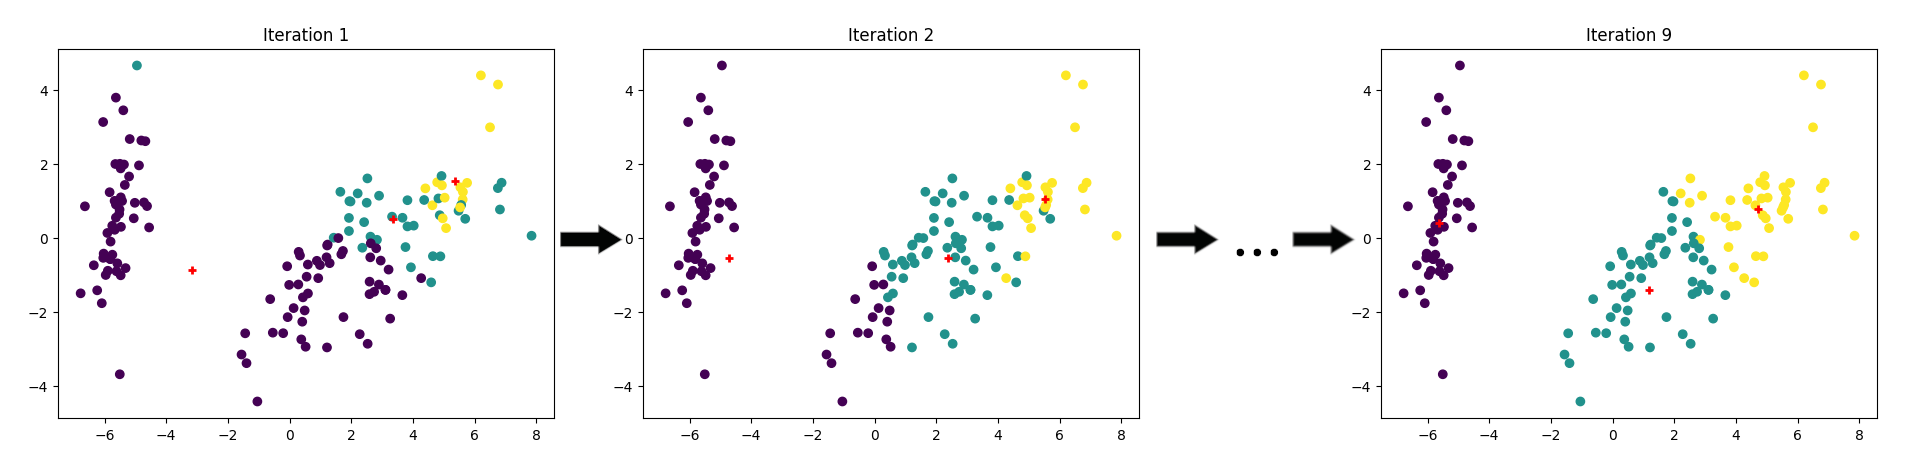
\includegraphics[width=0.7\textwidth]{demo_kmeans_iris.png}
  \label{fig:kMeansDemoIris}
\end{figure}

É importante entender também as limitações do algoritmo k-means. Como explicitado anteriormente, não há garantias de que o processo encontre o melhor agrupamento possível para o conjunto de dados, apenas o melhor possível a partir dos centroides iniciais.

O algoritmo também é sensível a \textit{outliers}, isto é, pontos de dados que se diferem muito da distribuição geral dos dados. A presença destes pode causar grandes deformações dos clusters --- basicamente \enquote{puxando} os centroides para mais perto dos \textit{outliers}.

Um dos argumentos necessários na chamada do algoritmo é considerado também uma limitação: o parâmetro $K$. Como é necessário que o k-means seja informado da quantidade de agrupamentos a serem feitos, isso implica que já se saiba algo a respeito da natureza ou geometria do conjunto de dados a ser agrupado, o que nem sempre é possível, ainda mais para datasets de alta dimensionalidade, onde uma visualização útil para se interpretar os dados se torna extremamente difícil.

Mesmo com todas essas limitações, o k-means continua um algoritmo ubíquo em diversas áreas da computação, como discutido a seguir, e segue sendo amplamente estudado e aprimorado na literatura.

% * ##########################

\subsection{Aplicações Reais}

O k-means, reconhecido por sua simplicidade e eficácia, é empregado em uma variedade de aplicações práticas em diversos campos. Sua capacidade de efetivamente segmentar dados em grupos com características similares o torna uma ferramenta versátil para diversos usos, desde análises de mercado até sistemas de recomendação.

Uma das aplicações mais comuns do k-means é a segmentação de clientes. Nesse contexto, empresas de diversos setores, como bancos, telecomunicações, e-commerce e publicidade, utilizam o k-means para agrupar clientes com base em comportamentos de compra, preferências ou demografia, permitindo o desenvolvimento de estratégias de marketing direcionadas e personalizadas. Esta aplicação não apenas ajuda as empresas a entender melhor seus clientes, mas também a otimizar suas ofertas e serviços de acordo com as necessidades de cada segmento.

Um exemplo concreto dessa aplicação é a realizada em um estudo de caso de 2018 \cite{kMeansSupplierRiskAss2018}, que utilizou o k-means para avaliar não clientes, mas sim realizar a análise de risco de fornecedores comerciais.

Neste estudo, o método k-means foi aplicado para \textbf{avaliar e segmentar fornecedores} de uma empresa de maquinário pesado com base em seus perfis de risco. A metodologia incluiu a utilização do Best-Worst Method (BWM) para determinar os pesos de 17 critérios de risco, seguido pela aplicação de Análise de Fatores para redução de dimensionalidade dos dados de risco, resultando em quatro fatores principais. Utilizando esses fatores, o k-means foi empregado para dividir os fornecedores em três clusters, representando diferentes níveis de exposição ao risco, o que permitiu uma análise detalhada das características de risco de cada grupo.

Os resultados do estudo demonstraram que a abordagem baseada em k-means é eficaz para a categorização dos fornecedores em grupos homogêneos quanto aos riscos enfrentados, fornecendo insights significativos para a gestão e o avaliação de fornecedores. Este agrupamento facilitou decisões estratégicas na gestão de riscos, destacando a importância e utilidade de métodos analíticos avançados em ambientes empresariais competitivos. O estudo sugere que a aplicação de técnicas de agrupamento de dados, como o k-means, pode melhorar significativamente as práticas de compra e a gestão de riscos em setores industriais.

Outra aplicação notável do k-means é na organização e classificação de documentos. Por exemplo, em grandes conjuntos de dados de texto, como coleções de artigos ou relatórios de pesquisa, o k-means pode agrupar documentos com temas ou conteúdos semelhantes, facilitando a gestão e a recuperação de informações. Este uso é particularmente valioso em campos como pesquisa acadêmica, onde a capacidade de navegar rapidamente por vastas quantidades de literatura é crucial.

Um exemplo específico dessa aplicação é explorado na documentação da biblioteca Python \textbf{Scikit Learn} \cite{kMeansDocClustering2024}. Nesse exemplo de implementação, é explorado o \textbf{agrupamento de documentos de texto} utilizando o método k-means com a biblioteca scikit-learn, focando em agrupar textos por tópicos de maneira eficaz. Ele emprega duas variantes do algoritmo k-means implementadas na biblioteca, o \textit{KMeans} e \textit{MiniBatchKMeans}, e utiliza a Análise Semântica Latente (LSA) para a redução de dimensionalidade e a identificação de padrões \enquote{escondidos} nos dados. Além disso, são utilizados dois métodos de vetorização de texto: \textit{TfidfVectorizer} e \textit{HashingVectorizer}, que ajudam na transformação do texto em uma representação numérica que pode ser usada pelo algoritmo de agrupamento.

Para a análise, o dataset \textit{20 newsgroups} é utilizado, selecionando quatro tópicos para manter o custo computacional acessível e melhorar a clareza do problema de agrupamento, removendo metadados desnecessários como cabeçalhos e citações. A eficácia do agrupamento é avaliada através de várias métricas, incluindo homogeneidade, completude, medida-V, índice Rand ajustado e coeficiente de silhueta, destacando que a aplicação da técnica de LSA antes do agrupamento melhora significativamente tanto a estabilidade quanto a qualidade dos clusters. Esses resultados ilustram o potencial dessas técnicas para categorizar e entender grandes conjuntos de dados de texto, proporcionando insights valiosos sobre a organização dos tópicos dentro dos documentos.

O k-means também tem aplicações significativas no processamento de imagens, como na segmentação de imagens, onde o algoritmo agrupa pixels semelhantes para identificar e separar diferentes objetos ou regiões dentro de uma imagem. Esta técnica é amplamente utilizada em tarefas como reconhecimento de padrões, visão computacional e até mesmo na melhoria de algoritmos de compressão de imagem, tornando-a uma ferramenta fundamental na era digital.



% * ####################################

% \section{Algoritmo 2: Hierarchical Clustering}

% \textbf{Escrever uma sub-seção sobre o Hierarchical Clustering, no mesmo estilo da seção do k-means. Seção opcional, só fazer depois de concluir TODO o resto do k-means + seus experimentos + resultados + código.}





% * ############################################################################
\chapter{Levantamento do Estado da Arte}
% * ############################################################################

No contexto histórico, o aumento exponencial no volume de dados gerados e armazenados digitalmente tornou-se uma realidade desde as últimas décadas do século XX. Com o advento da internet, mídias sociais, dispositivos inteligentes e sensores, a quantidade de dados disponíveis cresceu exponencialmente. Esses dados não estruturados, em sua maioria, requerem técnicas avançadas para extrair informações valiosas e úteis \cite{dataMining2012-preface}.

Nesse cenário, os algoritmos de agrupamento emergem como uma ferramenta essencial para entender a estrutura subjacente dos dados, identificar padrões, segmentar clientes, recomendar produtos e até mesmo na medicina para classificar pacientes com base em características semelhantes. No entanto, à medida que os conjuntos de dados crescem em escala e complexidade, a eficiência computacional torna-se uma preocupação crítica.

A necessidade de processamento mais rápido de grandes conjuntos de dados é evidente. Os algoritmos de agrupamento, especialmente quando aplicados a conjuntos de dados volumosos, podem se tornar computacionalmente intensivos e demandar uma quantidade considerável de tempo de execução. Isso não apenas limita a capacidade de análise em tempo hábil, mas também impõe restrições sobre a escalabilidade das soluções de análise de dados.

Portanto, surge a necessidade de paralelizar esses algoritmos, aproveitando o poder computacional de sistemas distribuídos, clusters de computadores ou arquiteturas de hardware com múltiplos núcleos. A paralelização não apenas acelera o processo de agrupamento, mas também permite lidar com conjuntos de dados cada vez maiores, garantindo que as análises permaneçam viáveis e eficientes em um cenário de big data.

As pesquisas aqui resumidas buscam explorar a história da paralelização de algoritmos de agrupamento, destacando os avanços significativos nesta área e sua importância contínua na era da análise de enormes volumes de dados. Este segmento do trabalho serve como uma ponte entre o passado e o presente, ilustrando não apenas estudos mais antigos que formaram uma base teórica e prática na áreal, mas também como a introdução das (GPUs) transformou fundamentalmente este campo. Ao revisitar os marcos históricos, é possível delinear o caminho de inovações e aprimoramentos que permitiram a jornada até a era atual, onde a paralelização possibilita o processamento de conjuntos de dados de magnitude anteriormente inimaginável com eficiência e rapidez sem precedentes.

% ?
% ? Concluindo...
% ?

Como evidenciado nas seções seguintes, a avaliação dos estudos recentes sobre a paralelização de algoritmos de agrupamento, especialmente os que utilizam a plataforma CUDA para implementá-los em GPUs NVIDIA, revela avanços significativos tanto na eficiência quanto na utilidade prática dos processos de agrupamento. Estas melhorias são notáveis em aplicações que variam desde o processamento de imagens até a física de alta energia.

Os avanços na utilização de processadores vetoriais para paralelização têm demonstrado que é possível obter reduções significativas nos tempos de processamento, mantendo, ou até mesmo melhorando, a qualidade dos resultados destes tipos de algoritmos.

No entanto, apesar dos avanços significativos, ainda existem lacunas importantes a serem preenchidas. Uma das principais lacunas é a falta de algoritmos paralelos que sejam eficientes para diferentes tipos e tamanhos de conjuntos de dados. Outra área que merece atenção é a escalabilidade dos algoritmos paralelizados. À medida que os conjuntos de dados continuam a crescer em tamanho e complexidade, torna-se crucial que os algoritmos de agrupamento possam escalar eficientemente para atender a essas demandas crescentes.

% ?
% ?
% ? A palavra "escalar" pode ser usada assim no português mesmo? Eu encontrei uns exemplos na WikiPédia, mas também parece ser utilizada a palavra "escalonar" ao invés. Qual o mais correto?
% ?
% ?

Direções futuras na pesquisa podem incluir o desenvolvimento de algoritmos paralelos que sejam mais adaptáveis a diferentes tipos e tamanhos de dados, além da integração de técnicas de aprendizado de máquina para melhorar a precisão e eficiência dos processos de agrupamento. Além disso, pode ser útil explorar mais a fundo o potencial das novas arquiteturas de GPU e outras plataformas de computação paralela, como as TPUs e FPGAs (vide o capítulo \ref{ssc:vetorial}), para avançar ainda mais na paralelização destes algoritmos.

A exploração de técnicas híbridas, que combinem métodos de agrupamento clássicos com novas abordagens baseadas em aprendizado profundo (\textit{Deep Learning}), também pode oferecer caminhos promissores para melhorar tanto a velocidade quanto a qualidade dos algoritmos. Finalmente, há uma necessidade contínua de pesquisa que aborde questões de eficiência energética e sustentabilidade ambiental no contexto da computação de alto desempenho aplicada ao agrupamento de dados.



% * ####################################

\section{Primeiras Implementações Paralelas}

A ideia de acelerar a execução de algoritmos de agrupamento de dados utilizando a computação paralela não é nova. Desde o advento das pesquisas envolvendo tais processos e do aumento cada vez mais rápido de volume de dados disponíveis para análise, vem-se fazendo evidente a necessidade de otimizar ao máximo esses algoritmos.

Um dos estudos mais antigos encontrados que tenta paralelizar um algoritmo desse tipo é o \enquote{\textit{Parallel K-means Clustering Algorithm on NOWs}} \cite{kMeansParallelkantabutra2000}.

Nesse artigo, é apresentada uma abordagem para melhorar a eficiência do \textbf{algoritmo k-means} através da paralelização. O objetivo principal é reduzir a complexidade temporal do algoritmo k-means serial aplicando teorias de computação paralela, alcançando uma melhoria de um fator de $O(K/2)$, onde $K$ é o número de clusters desejados. Além disso, visa permitir que o algoritmo seja executado em uma memória coletiva maior, composta por várias máquinas, superando a limitação de memória de uma apenas uma, o que permite escalar o tamanho do problema em até $O(K)$ vezes o tamanho que poderia ser processado em uma única máquina.

A pesquisa foi realizada utilizando uma rede de estações de trabalho homogêneas com uma rede Ethernet e a comunicação entre processos foi feita por meio da Interface de Passagem de Mensagens (MPI). O método proposto usa uma abordagem mestre-escravo (\textit{master-slave}) onde um processo mestre distribui subconjuntos de dados para processos escravos, que calculam médias locais e participam de um processo iterativo de realocação de pontos de dados para minimizar uma função de erro quadrático. A análise de complexidade de tempo e espaço foi detalhadamente realizada, destacando a eficiência do algoritmo paralelizado em comparação com sua versão serial.

Os resultados experimentais mostraram que, para conjuntos de dados grandes (mais de 700.000 datapoints), a versão paralela do algoritmo conseguiu obter uma melhoria significativa na velocidade de execução, evidenciada por um "speedup" de até O(K/2) conforme o tamanho do problema aumenta. Isto foi particularmente notável quando o tamanho do problema excedeu a capacidade de memória de uma única máquina, um cenário onde a versão serial do algoritmo não pôde sequer ser executada.

No fim, a pesquisa demonstra que a paralelização do algoritmo k-means em uma rede de estações de trabalho oferece uma melhoria significativa tanto em termos de complexidade temporal quanto de escalabilidade do tamanho do problema, alcançando uma eficiência de 50\% na redução do tempo de complexidade. Esta eficiência é considerada alta para a época e dada a natureza global do algoritmo k-means e o uso de um sistema baseado em passagem de mensagens Ethernet. O trabalho sugere que futuras pesquisas poderiam focar na redução do tempo de comunicação ou na adaptação do algoritmo para funcionar com um número flexível de máquinas, visando melhorias ainda maiores na eficiência e escalabilidade.

Outro estudo antigo que mostra o início das tentativas de paralelizção de algoritmos de agrupamento é o \enquote{\textit{Parallel K-Means Algorithm on Distributed Memory Multiprocessors}} \cite{parallelKMeansJoshi2003}. Aqui, é explorada uma \textbf{implementação paralela do k-means}, visando acelerar o agrupamento de grandes conjuntos de dados em um cluster de \textit{workstations} da Sun Microsystems. A pesquisa objetiva explorar o paralelismo de dados inerente ao k-means, utilizando o modelo de passagem de mensagens para dividir o conjunto de dados entre processos, buscando reduzir o tempo total de computação.

O algoritmo implementado no estudo divide o conjunto de dados entre os processos de um sistema de memória distribuída, onde cada processo é responsável por uma parte dos dados. Esta abordagem visa calcular a associação datapoint-cluster para cada partição de forma mais rápida. A comunicação entre os processos, embora necessária para a recomputação dos centróides e a avaliação da qualidade dos clusters, representa um custo significativo, especialmente para conjuntos de dados menores, onde o tempo de comunicação domina em relação ao tempo de processamento dos dados. A pesquisa destaca a importância de minimizar essa comunicação para melhorar a eficiência do algoritmo paralelo.

A implementação utiliza o modelo de Programa Único Múltiplos Dados (SPMD) e a Interface de Passagem de Mensagens (MPI) para a comunicação entre processadores. Inicialmente, o processo raiz calcula os centróides iniciais e os transmite a todos os outros processos. Cada processo então computa distâncias, atribui pontos ao centróide mais próximo, e calcula erros quadráticos médios locais. Essas operações são repetidas até a convergência, com processos recomputando centróides e avaliando a qualidade global do agrupamento.

Embora a paralelização tenha mostrado benefícios, como a distribuição eficiente do processamento e a possibilidade de lidar com conjuntos de dados maiores, o ganho de velocidade ótimo não foi alcançado devido ao custo sequencial associado à escolha dos centróides iniciais e à influência de outliers na formação dos clusters. A pesquisa sugere que futuros trabalhos podem explorar a paralelização em multiprocessadores de memória compartilhada, abordar questões de valores ausentes e outliers, e testar variantes probabilísticas do k-means ou o algoritmo K-modes para conjuntos de dados categóricos de grande escala.

Esse estudo demonstra o potencial e os desafios da paralelização do k-means para o agrupamento de dados em grandes escalas, tendo aberto caminho para pesquisas futuras voltadas à otimização da eficiência e da capacidade de processamento desses algoritmos em ambientes de computação de alta performance, para a época.

Ambos dos últimos dois estudos comentados predatam implementações em GPU de algoritmos de agrupamento de dados, demonstrando tentativas de paralelização com outras técnicas além da área de GPGPU, usando técnica como a computação distribuída, processamento paralelo SIMD, entre outras.

Para explorar as primeiras implementações de algoritmos de agrupamento que utilizaram especificamente placas de vídeo para paralelização é preciso avançar ao menos um ano na linha do tempo.

O estudo mais antigo encontrado a utilizar essa técnica é o \enquote{\textit{GPU Acceleration of Iterative Clustering}} \cite{iterativeClusteringGPU2004}. Esse estudo apresenta uma abordagem inovadora para \textbf{acelerar algoritmos iterativos de agrupamento}, como o \textbf{k-means} e a \textbf{Análise de Componentes Principais Agrupada (CPCA)}, utilizando o poder computacional das unidades de processamento gráfico. A pesquisa destaca o potencial das GPUs não apenas para gráficos e renderização, mas também para acelerar algoritmos amplamente utilizados em campos como visão computacional, processamento de sinais, compressão de dados e geometria computacional. O foco é na utilização da arquitetura de streaming de alta performance das GPUs para executar a parte mais custosa computacionalmente desses algoritmos, resultando em acelerações significativas.

O método proposto utiliza a arquitetura das GPUs para realizar as avaliações métricas, que são a parte mais intensiva em termos de cálculos dos algoritmos de agrupamento. Os autores desenvolveram uma versão hierárquica do algoritmo k-means, projetada para aumentar o paralelismo SIMD, resultando em um desempenho melhorado em comparação com abordagens hierárquicas tradicionais do k-means, que podem não aproveitar totalmente o hardware das GPUs. A GPU lida com a tarefa de particonamento dos dados, enquanto a CPU é responsável por atualizar os modelos de cada cluster, otimizando o uso dos recursos computacionais disponíveis.

Nos resultados apresentados, a aceleração obtida varia entre 1,5 a 3 vezes em comparação com a execução apenas na CPU, dependendo do tamanho do conjunto de dados. Este aumento de desempenho é particularmente relevante para datasets grandes e métricas complexas, onde a aceleração permite soluções mais rápidas e viáveis para problemas que antes eram proibitivamente lentos para resolver. O estudo também discute as limitações atuais e potenciais futuras melhorias, incluindo a implementação de etapas de atualização do modelo diretamente nas GPUs, o que poderia reduzir ainda mais o tempo de computação.

No fim, o trabalho demonstra o potencial das GPUs para acelerar significativamente algoritmos de agrupamento iterativos, abrindo caminho para aplicações interativas e em tempo real que antes não eram possíveis. As futuras direções de pesquisa sugeridas incluem a exploração de métodos para minimizar a comunicação entre a GPU e a CPU e expandir a aplicabilidade dessa abordagem para métricas de agrupamento que não podem ser avaliadas independentemente para cada ponto. Este estudo não apenas destaca a utilidade das GPUs além da área gráfica, mas também promove a investigação contínua para explorar plenamente suas capacidades para acelerar uma gama ainda mais ampla de algoritmos computacionais.


% * ####################################

\section{K-means e Variantes}

Partindo para estudos mais recentes, representando o estado da arte da área, e focando mais no k-means e suas diversas variantes, é de destaque o estudo \enquote{\textit{Parallelization of Partitioning Around Medoids} [\dots]} \cite{pamKMedoids2020}, onde os autores propuseram uma implementação paralela do \textbf{algoritmo de agrupamento K-Medoids}, especificamente da sua versão conhecida como \textbf{PAM (\textit{Partitioning Around Medoids})}, que é utilizada para dividir conjuntos de dados em clusters de forma que minimizem as distâncias internas. Esta versão paralela foi desenvolvida para ser executada em Unidades de Processamento Gráfico (GPUs) utilizando a arquitetura CUDA da NVIDIA.

O principal desafio do K-Medoids reside em seu alto custo em tempo de execução e em uso de espaço de memória, especialmente para grandes conjuntos de dados, o que pode tornar sua aplicação inviável em contextos práticos. Para superar esses empecilhos, os autores optaram por uma abordagem paralela, implementada em CUDA, e que não necessita do pré-cálculo de uma tabela completa de distâncias, algo quase onipresente em implementações anteriores do K-Medoids, reduzindo assim o consumo de memória e acelerando muito o processo de execução.

Os resultados foram promissores, demonstrando que a versão paralelizada em GPU do algoritmo PAM conseguiu uma melhoria significativa de desempenho em comparação com as implementações tradicionais em CPU e até mesmo com implementações em Matlab --- ambas estas utilizam a tabela de distâncias pré-calculada, custosa em uso memória. Especificamente, o estudo relatou um aumento de velocidade de 11 a 15 vezes em relação à implementação em CPU, e de 2 a 3 vezes em relação ao Matlab, para grandes volumes de dados.

Este avanço indica que o algoritmo K-Medoids, adaptado para uso altamente paralelizado em GPUs, torna-se uma alternativa mais viável para o agrupamento de grandes conjuntos de dados, oferecendo melhorias tanto em termos de tempo de execução quanto na capacidade de lidar com muitos pontos de dados sem exigir quantidades excessivas de memória. Portanto, a pesquisa contribui significativamente para a área de mineração de dados e aprendizado de máquina, abrindo novas possibilidades para o uso eficiente do K-Medoids em aplicações práticas de big data.



% * ####################################

\section{Algoritmos Hierárquicos}

O \textbf{Agrupamento Aglomerativo Paralelo} é uma técnica fundamental no campo da mineração de dados e aprendizado de máquina, especialmente quando lidamos com grandes conjuntos de dados. Tradicionalmente, os \textbf{algoritmos de agrupamento aglomerativo} (\textbf{HAC}, em inglês), conhecidos por sua abordagem hierárquica, eram limitados pela capacidade computacional e de memória das máquinas. Com a evolução da computação paralela, surgiu a necessidade de adaptar estes algoritmos para ambientes onde múltiplos processos podem ser executados simultaneamente, melhorando significativamente a eficiência e a escalabilidade do agrupamento de grandes quantidades de instâncias.

Antes do desenvolvimento do algoritmo k-means, um dos métodos de agrupamento mais populares, havia um forte interesse no agrupamento aglomerativo devido à sua capacidade de revelar a estrutura hierárquica dos dados. No entanto, sua aplicação era bastante limitada devido ao alto custo computacional e à demanda por grandes quantidades de memória. A paralelização do agrupamento aglomerativo surgiu como uma solução para essas limitações, permitindo o processamento de dados em grande escala de uma maneira mais viável.

Um avanço significativo no Agrupamento Aglomerativo Paralelo foi realizado através do desenvolvimento do \textbf{framework ParChain}, discutido no artigo \enquote{\textit{ParChain: A Framework for Parallel Hierarchical} [\dots]} \cite{parChainHAC2021}. O ParChain propõe uma estrutura para projetar algoritmos paralelos de agrupamento hierárquico aglomerativo que utilizam memória linear, em contraste com a memória quadrática requerida pelos algoritmos paralelos anteriores. Baseado na paralelização do algoritmo de cadeias de vizinhos mais próximos, o ParChain permite que múltiplos clusters sejam mesclados em cada rodada, melhorando a eficiência e a escalabilidade do processo de agrupamento.

O estudo demonstrou que implementações altamente otimizadas do ParChain, utilizando 48 núcleos com \textit{hyper-threading} bidirecional, alcançaram uma aceleração significativa em comparação com os algoritmos paralelos HAC de última geração. Mais especificamente, observou-se uma aceleração entre 5,8--110,1 vezes no tempo de execução, além de uma redução de até 237,3 vezes no espaço necessário. Assim, o framework foi capaz de escalonar para tamanhos de conjuntos de dados com dezenas de milhões de pontos --- um feito que os algoritmos existentes não conseguiam alcançar.

A introdução do HAC paralelo, e particularmente do framework ParChain, marcou um ponto de virada na análise de dados em grande escala, permitindo a exploração de estruturas de dados complexas de maneira mais eficiente e profunda. Este desenvolvimento não apenas superou as limitações dos métodos de agrupamento anteriores, mas também abriu novas avenidas para pesquisas futuras, incluindo a otimização de outros critérios de ligação (entre pontos de dados e grupos) e a aplicação em diferentes domínios de dados.



% * ####################################

\section{Outras Pesquisas Relevantes}

\textbf{TODO: Escrever um parágrafo introdutorio básico aqui?}

% TODO
% TODO
% TODO: Vide acima
% TODO
% TODO

O estudo \enquote{\textit{CLUE: A Fast Parallel Clustering Algorithm for} [\dots]} \cite{clueParallelAlgo2020} expõe um \textbf{novo algoritmo de agrupamento} chamado \textbf{CLUstering of Energy (CLUE)}, destinado a otimizar o processo de agrupamento em calorímetros de alta granularidade utilizados em física de alta energia. O algoritmo foi projetado para ser totalmente paralelizável e eficiente, lidando com um grande número de \enquote{hits} ou detecções de depósitos de energia, que podem variar em número a cada detecção numa faixa entre milhares a milhões, dependendo da granularidade e do número de partículas que entram no detector.

O CLUE utiliza uma abordagem baseada em densidade para o agrupamento, calculando duas variáveis-chave para cada ponto: a densidade local e a separação. Utiliza também um índice espacial de grade fixa para acelerar a consulta de vizinhos, atribuindo todos os pontos de dados a quadrantes de uma malha, tornando o processo de busca por vizinhos mais rápido e escalável. Além disso, o algoritmo pode efetivamente identificar e agrupar formatos de clusters não-esféricos e rejeitar ruídos, adaptando-se às necessidades específicas da análise de dados em calorímetros.

A implementação do CLUE em GPUs mostrou ser significativamente mais rápida do que as implementações em CPU de thread único, alcançando um aumento de velocidade de 48 a 112 vezes, dependendo do número de pontos processados. Esse desempenho é crucial para a reconstrução de eventos em física de partículas, onde o tempo de processamento é limitado e grandes volumes de dados precisam ser analisados rapidamente.

O estudo confirmou que o algoritmo CLUE é altamente escalável, mantendo um desempenho linear em relação ao número de pontos de entrada, o que é ideal para o tratamento de dados provenientes de calorímetros de alta granularidade, como os previstos para o CMS no LHC de alta luminosidade.

Este desenvolvimento representa um avanço significativo na análise de dados em física de alta energia, permitindo um processamento de dados mais rápido e eficiente, o que é essencial para explorar o potencial completo de futuros experimentos de física de partículas.

Outro estudo muito relevante é o \enquote{\textit{Evaluation of Clustering Algorithms on GPU-Based Edge Computing Platforms}} \cite{edgeComputingGPUsIOT2020}, que analisou a viabilidade de executar algoritmos de agrupamento de dados, computacionalmente exigentes, em \textbf{plataformas de computação de borda} (\textbf{\textit{Edge Computing}}, uma abordagem que permite computação distribuída de baixo custo computacional nas bordas de uma rede, o mais próximo possível do cliente) equipadas com GPUs de baixo consumo. Foram testados três algoritmos de agrupamento diferentes: \textbf{K-means}, \textbf{Fuzzy Minimals (FM)} e \textbf{Fuzzy C-means (FCM)}, em dois contextos: \textbf{computação de alto desempenho (HPC)} e computação de borda.

Os resultados mostraram que, ao usar as GPUs em plataformas de borda como a NVIDIA AGX Xavier, foi possível obter uma aceleração significativa em comparação com as versões sequenciais dos algoritmos rodando nas próprias plataformas de borda. Especificamente, observou-se um aumento de velocidade de até 11 vezes para os códigos GPU em relação às versões sequenciais. Além disso, comparando as plataformas de computação de borda com as plataformas HPC, houve economias de energia de até 150\% ao usar a computação de borda em vez da versão HPC.

Portanto, este estudo concluiu que as plataformas de computação de borda equipadas com GPUs de baixo consumo oferecem uma alternativa viável e muito mais energeticamente eficiente para a execução de algoritmos de agrupamento de dados pesados. Isso abre novas possibilidades para aplicativos de IoT avançados, onde a análise de dados pode ser realizada mais perto da fonte de dados, reduzindo a latência e o consumo de energia associados à transmissão de grandes volumes de dados para a nuvem ou outros centros de dados remotos.

Além disto, é destacado no estudo que essas melhoras de desempenho possivelmente possibilitarão a análise de dados considerados como \textit{dark data}: enormes volumes de dados gerados diariamente por dispositivos IoT que costumavam nunca ser de fato analisados. Essa interpretação \enquote{inédita} dos dados iria possibilitar a criação de aplicações mais inteligentes numa nova geração de dispositivos IoT, beneficiando a sociedade.





% * ############################################################################
\chapter{Metodologia de Desenvolvimento e Pesquisa}
% * ############################################################################

% \textbf{TODO: Adicionar em algum lugar desse capítulo uma figura, um diagrama, explicativo sobre a metodologia usada para parelelizar um algoritmo de agrupamento genérico. Vide arquivo \enquote{..\textbackslash Notes\_230922\_171133.pdf}.}

% TODO
% TODO
% TODO Vide acima. Local do arquivo referenciado: ..\Notes_230922_171133.pdf
% TODO
% TODO

A pesquisa realizada neste trabalho consistiu de estudos e análises de trabalhos prévios, desenvolvimento de uma versão paralelizada do algoritmo de clustering k-means e experimentos sobre essa implementação. Pode-se dividir tal metodologia em um conjunto de etapas que foram realizadas.

A \textbf{primeira etapa} consistiu em uma extensa pesquisa bibliográfica. O intuito é levantar o estado da arte na área de algoritmos de agrupamento acelerados com técnicas de paralelismo, como implementações em GPU. O foco foi entender quais algoritmos já foram implementados paralelamente com sucesso, e como foram feitas tais implementações, além dos ganhos em desempenho destas. Essa etapa permitiu agregar conhecimento sobre como utilizar ferramentas como a biblioteca CUDA para acelerar algoritmos de agrupamento, além de mostrar uma prévia da magnitude de ganho de desempenho esperado de uma paralelização média desse tipo de algoritmo.

A \textbf{segunda etapa} consistiu na implementação de duas versões, uma serial e uma paralela, de um dos mais antigos e conhecidos algoritmos de agrupamento de dados: o \textbf{k-means}. A função dessa etapa da pesquisa foi aprender como programar, na prática, um algoritmo de agrupamento e, depois, como paralelizá-lo utilizando a biblioteca Python \textit{Numba} --- que utiliza a plataforma CUDA, internamente. Por ser um algoritmo mais antigo, o k-means já foi muito estudado anteriormente, tanto em versões seriais quanto paralelas, com grande presença na bibliografia da área. Assim, a implementação aqui foi facilitada pelo grande acúmulo de conhecimento bibliográfico. % Os ganhos de velocidade da versão paralela foi então comparada também com os ganhos obtidos nos trabalhos analisados na primeira etapa. Isso serviu como uma validação da corretude da implementação feita.

% A \textbf{terceira etapa} consistiu na implementação de uma versão paralela um pouco mais \enquote{inédita} de algum algoritmo de agrupamento, ou seja, um algoritmo cuja implementação paralela foi raramente estudada à fundo em pesquisas. O algoritmo escolhido para essa etapa foi o de \textbf{Agrupamento Hierárquico}. Usando o aprendizado adquirido nas etapas anteriores, este algoritmo foi paralelizado em Python, utilizando novamente a biblioteca \textit{Numba}, e seus resultados comparados com a versão serial (rodando somente em uma thread, na CPU) para garantir corretude.

A \textbf{terceira etapa} consistiu na busca de um procedimento geral para paralelizar um algoritmo de agrupamento genérico. Ou seja, o foco foi encontrar um passo-a-passo de identificação de possíveis modificações no código de um algoritmo serial que, ao fim, pudesse transformá-lo numa versão acelerada, usando CUDA, ainda mantendo sua corretude e proporcionando algum ganho significativo de desempenho.

A \textbf{quarta etapa}, por fim, consistiu em diversos experimentos de ganho de velocidade, ou \textit{speedup}, do k-means, que teve aqui sua versão acelerada em GPU implementada e apresentada. Os resultados desses experimentos proporcionaram uma boa visão da magnitude do ganho de desempenho ao paralelizar algoritmos de agrupamento usando CUDA, além de outros conhecimentos, como saber se há um teto ou chão para tais ganhos, como o \textit{speedup} aumenta ou diminui com o crescimento do número de datapoints ou variáveis no conjunto de dados a ser analisado, e também como outros parâmetros importantes que não sejam velocidade são afetados, como a precisão dos resultados gerados pelo k-means, pois não há serventia em ganhar grande velocidade enquanto se perde o propósito de se agrupar dados em primeiro lugar, que é a capacidade de encontrar informações reais úteis em grandes datasets.



% * ####################################

\section{Identificando o Potencial de Paralelismo}
\label{chp:identifPotencParalel}

Antes de se iniciar qualquer implementação que busque ganhar desempenho com o paralelismo, é crucial realisar uma análise para encontrar quais partes de um processo sequer podem ser paralelizadas e quais são necessariamente seriais --- isto é, precisam ser realizadas sequencialmente, sem processamentos simultâneos para aceleração.

Evidentemente, nem todo processo pode ser paralelizado. Há requisitos importantes para que uma tarefa possa ser executada de maneira paralela. Primeiro, é necessário que a tarefa possa ser subdivida em diversas outras tarefas menores. Segundo, é necessário que essas tarefas sejam independentes entre si, isto é, que a execução de uma não dependa diretamente do resultado de outra.

Um exemplo de tarefa facilmente paralelizável, como exibido nos Capítulos \ref*{ssc:implementaçãoCUDA} e \ref*{ssc:implementaçãoNumba}, é a soma de dois vetores. Para dois vetores de tamanho $N$, é possível calcular a soma deles paralelamente, calculando a soma de cada par de elementos, um de cada vetor, simultaneamente. Isso é possível pois, para dois vetores $x$ e $y$, a soma dos elementos $x[i]$ e $y[i]$ não depende da soma dos elementos $x[i+1]$ e $y[i+1]$.

Já um exemplo de uma tarefa inerentemente serial seria o hashing consecutivo de um dado, uma operação onde é calculado o hash de uma mensagem $N$ vezes, cada vez aplicando a operação de hashing novamente sobre o valor gerado pela operação anterior. Para calcular a terceira operação de hash do dado, é estritamente necessário que o hash da segunda operação tenha sido calculado, que por sua vez necessita que a primeira operação de hashinh tenha sido concluída. A paralelização num cenário desses é impossível, pois o resultado de uma sub-tarefa depende de outra, impedindo que sejam executadas simultaneamente.

A identificação de trechos altamente paralelizáveis do algotimo k-means é simples. Abaixo, há um excerto do pseudocódigo que descreve seu processo, exibido por completo no Capítulo \ref{sec:kMeans} (Algoritmo \ref{code:kMeans.pseudo}).

\codeexternal[
  language=,
  firstline=8,
  lastline=12,
  mathescape,
  numbers=none,
  label=code:kMeans.snippet1.pseudo,
  % caption={Implementação padrão em pseudocódigo do k-means},
]{code-snippets/kMeans.pseudo}

É simples perceber que os trechos com maiores potenciais de paralelização são o passo 2.1 e o 2.2.

No passo 2.1, temos o cálculo de todas as distâncias euclidianas entre cada um dos $N$ elementos do dataset e os $K$ centroides de cada grupo. Ou seja, um mesmo cálculo é realizado um total de $N \cdot K$ vezes a cada iteração do algoritmo. Cada um dos cálculos das distâncias independe dos outros, então essa grande operação pode ser altamente paralelizada.

No passo 2.2, o cálculo dos novos centroides é realizado. Essa operação requer a redução de um vetor bidimensional de dimensões $N \cdot D$ em um vetor unidimensional de tamanho $D$. Essa redução é feita com a soma de todas as coordenadas dos datapoints mais próximos do centroide atualmente sendo recalculado e depois a divisão do valor final pelo número de datapoints que foram somados, realizando efetivamente uma média das coordenadas dos pontos de um grupo, para encontrar o novo centroide do grupo. Novamente, é uma operação de $(N_c - 1) \cdot D$ somas, onde $N_c$ é o número de pontos de dados no grupo cujo centroide está sendo recalculado, com $D$ divisões no final para encontrar a média. Por ser uma operação de redução, onde a saída tem dimensionalidade menor que a entrada, há um grau de dificuldade maior na implementação de uma versão paralela, mas é perfeitamente possível, com subdivisões iterativas dos vetores.

Na verdade, até o passo 1 no pseudocódigo acima é paralelizável, já que a geração dos centroides aleatórios pode ser feita simultaneamente para os $K$ centróides. Porém, como $K$ quase sempre é muito menor que $N$ nos datasets, essa implementação costuma não valera a pena.

Uma parte do k-means que nunca poderia ser paralelizada são as operações entre cada itearação. Isto é, o passo 2.1 da teceira iteração nunca pode ser executado ao mesmo tempo que o mesmo passo 2.1 da segunda iteração do algoritmo. Isso pois a relação datapoint--centroide é passível de mudanças a cada iteração, e o cálculo das distâncias dos centroides numa iteração $i$ depende do cálculo das distâncias da iteração $i-1$, para qualquer $i > 1$.

% TODO
% TODO
% TODO: Se der tempo, apresentar a mesma ideia mas para o algoritmo do agrupamento hierárquico aqui!
% TODO
% TODO



% * ####################################

\section{Implementação do K-means}
\label{sec:kMeansImplementações}

Como detalhado no capítulo \ref{sec:kMeans}, o \textbf{k-means} é um dos mais importantes e amplamente utilizados algoritmos de agrupamento, mesmo com suas diversas limitações. Ele foi selecionado nessa pesquisa como exemplo inicial de paralelização de algoritmo por ser de fácil entendimento e possuir uma implementação relativamente simples.

Foram utilizadas bibliotecas Python renomadas na área de ciência de dados, como \textit{Numpy} e \textit{Pandas}, para facilitar a implementação e garantir uma execução altamente otimizada, visto que essas bibliotecas implementam chamadas em C/C++ para executar suas partes mais computacionalmente custosas, garantindo uma performance superior à chamadas de alto nível \cite{sciPyAndNumpy2012}.

Há duas importações imprescindíveis omitidas nos códigos exibidos neste capítulo, por motivos de brevidade. Uma é a da biblioteca Numpy, importada com o nome \textit{np}; a outra é a biblioteca Pandas, importada com o nome \textit{pd}.

É importante entender que há também um requisito de pré-processamento do conjunto de dados para essas implementações do k-means. Todas as variáveis devem ter seus valores normalizados. Esse processo é necessário para evitar que variáveis com amplitudes de valores maiores influenciem mais significativamente a construção dos clusters do que variáveis com amplitudes menores.

É recomendado, em geral, o método de \textit{normalização min-max} para algoritmos como o k-means, que utilizam a distância euclidiana para a construção de grupos \cite{standardizOfVars1988}. Este processo é explicado detalhadamente no capítulo \ref{sec:datasets}.

O \textbf{Algoritmo \ref{code:kMeansCPU}} abaixo é a implementação da versão serial, \textit{single thread}, do algoritmo k-means, usada nos experimentos descritos no capítulo \ref{chp:exp}.

\codeexternal[
  firstline=3,
  % lastline=,
  label=code:kMeansCPU,
  caption={Implementação serial do k-means},
]{code-snippets/kMeansCPU.py}

A função \textit{\codeinline{kMeansCPU}} declarada na linha 1 é uma implementação \enquote{concreta} do pseudocódigo apresentado no capítulo \ref{sec:kMeans}. Ela recebe o dataset com os dados a serem agrupados através de um dataframe do Pandas (variável \textit{\codeinline{dataset}}), além dos outros dois argumentos essenciais do k-means: o número de clusters \textit{\codeinline{k}} e o número de iterações máximas \textit{\codeinline{maxIter}}.

A primeira instrução a ser executada no algoritmo é a da linha 2, que inicializa os centroides usando valores aleatoriamente selecionados de dentro do conjunto de dados. Note que os centroides gerados não correspondem necessariamente a algum datapoint específico do dataset. Valores de qualquer datapoint podem ser selecionados e misturados para formar um centroide inicial. Isto é, pode existir um centroide inicial $C1 = (1.3, 2.3, 4.4, 3.7)$ mesmo não existindo nenhum datapoint com estes exatos valores no dataset. Em tal cenário, o valor da primeira variável poderia ter sido selecionado de um datapoint $d1 = (1.3, y1, z1, w1)$, enquanto o valor da terceira variável poderia ter originado de um datapoint $d2 = (x2, y2, 4.4, w2)$.

Após a inicialização dos centroides, são inicializadas outras variáveis importantes. Na linha 3 uma variável para armazenar os centroides da iteração anterior à atual é inicializado (\textit{\codeinline{centroids_OLD}}), como um dataframe vazio. Na linha 7 é inicializada uma variável de controle (\textit{\codeinline{iteration}}) para armazenar o índice da iteração, iniciando em 1.

Além disso, na linha 5 temos um pré-cálculo do logarítimo natural ($\ln{x}$) de todos os datapoints do dataset. Esses valores são usados mais adiante para facilitar o cálculo da média das variáveis de todos os datapoints de um certo cluster, isto é, na etapa de cálculo dos novos centroides a cada iteração.

Entramos então num laço de repetição (\textit{while loop}) na linha 9, onde o agrupamento dos dados é de fato realizado, iterativamente. Todo o restante do algoritmo é realizado dentro deste loop, exceto o retorno do resultado de classificação no final. A condição de parada é testada aqui, sendo ela (1) a iteração atual, ainda a ser realizada, ser maior que o número de iterações máximas (\textit{\codeinline{maxIter}}) ou (2) os centroides recém calculados serem exatamente iguais aos centroides calculados na iteração anterior --- o que significa que o agrupamento atual é o melhor que o algoritmo pode atingir nessa execução, ou seja, um máximo local. Como explicado no capítulo \ref{sec:kMeans}, o k-means não garante que os agrupamentos convirjam para um máximo global, apenas um máximo local.

Dentro do loop, a primeira instrução a ser executada é a de cálculo das distâncias. Isso é feito em uma só linha de código, a linha 10, utilizando largamente o poder de brevidade de código proporcionado pela biblioteca Pandas. O cálculo é realizado utilizando a distância euclidiana, aplicando a todos os centroides uma função lambda que, dado um centroide, calcula o quadrado das diferenças de todos os datapoints do dataset para este centroide. Ainda nessa função lambda, é calculada a raiz quadrada de cada resultado da operação anterior (usando a função \textit{\codeinline{sqrt}} da biblioteca Numpy) e, enfim, são somados os valores obtidos para cada variável de cada datapoint, gerando um valor final de distância para cada datapoint. No final, o resultado desse cálculo é um dataframe Pandas de dimensão $n \cdot k$, que é armazenado na variável \textit{\codeinline{distances}}. Assim, a linha $i$ desse dataframe possui $k$ valores $(dC1, dC2, \dots, dCk)$, onde $dCj$ é a distância do datapoint $i$ para o centroide de índice $j$ na lista de centroides.

Em seguida, na linha 11, é feita a associação de todos os datapoints com seus centroides mais próximos, utilizando o método \textit{\codeinline{idxmin}} do dataframe do Pandas, que aqui retorna, para cada datapoint, o índice da coluna com o menor valor. O resultado é armazenado na variável \textit{\codeinline{closestCent}}, e é um dataframe de dimensão $n \cdot 1$. Nesse dataframe, a linha $i$ possui apenas um valor $(j)$, onde $j$ é o índice do centroide $Cj$ mais próximo ao ponto $i$.

Na linha 12 um passo opcional de exclusão explícita da variável \textit{\codeinline{distances}} é realizado. Isso apenas informa ao coletor de lixo do Python que a variável pode ser descartada assim que for conveniente. Como a variável não é mais usada dentro do laço de repetição, a variável pode ser deletada sem problemas, liberando mais espaço em memória.

Na linha 14, os centroides usados para os cálculos de distância na iteração atual são salvos na variável \textit{\codeinline{centroids_OLD}}. Essa ação é imprescindível, pois é sempre necessário comparar os centroides gerados entre a iteração atual e a anterior a cada repetição do loop.

Na linha 15 finalmente é feito o cálculo dos novos centroides, após armazenar os centroides anteriores na variável \textit{\codeinline{centroids_OLD}} na linha 14. Novamente, assim como a operação da linha 10, temos uma cadeia de operações do Pandas. Utilizando o método \textit{\codeinline{groupby}} do objeto dataframe, agrupamos os logarítimos do dataset de acordo com a lista de centroides mais próximos. Isso gera $k$ sub-conjuntos de \textit{\codeinline{datasetLogs}}, cada um deles contendo apenas os logarítimos dos datapoints mais próximos a um certo centroide. Para cada um destes sub-conjuntos, é aplicada uma função lambda que, dado um sub-conjunto, calcula a média geométrica --- que, como discutido em mais detalhes no capítulo \ref{sec:kMeans}, é o único método correto para encontrar a média de valores normalizados \cite{geoMeanIsBetter1986} --- de todos os logarítimos dos datapoints do sub-conjunto. Essa cadeia de operações resulta em um dataframe de dimensão $d \cdot k$, onde $d$ é o número de variáveis que descrevem cada datapoint do dataset (\textit{features}). Esse dataframe é então transposto, acessando a propriedade \textit{\codeinline{T}} do dataframe, resultando em um novo dataframe final de dimensão $k \cdot d$, seguindo o mesmo formato usado na geração dos centroides iniciais e garantindo uma comparação correta entre os centroides de iterações consecutivas.

É importante notar que a operação supracitada do cálculo da média geométrica é realizada aqui utilizando uma operação alternativa, mas equivalente, à sua definição:

\[ \sqrt[n]{\displaystyle \prod_{i=1}^{n} a_{i}} \]

Sendo a operação equivalente:

\[ \exp{(\frac{1}{n} \cdot \displaystyle \sum_{i=1}^{n} \ln{a_{i}})} \]

Essa escolha foi feita pois é computacionalmente muito mais eficiente utilizar o exponencial ($e^{x}$) da média aritmética das somas dos logaritmos naturais dos $n$ elementos ao invés de utilizar a raiz $n$-ésima da multiplicação dos $n$ elementos. De fato, para datasets grandes com milhões de instâncias por cluster, seria inviável multiplicar tantos números e depois calcular a raíz $n$-ésima destes. Uma operação desse tipo necessitaria de quantidades exorbitantes de memória para armazenar o gigantesco resultado da multiplicação dessa miríade de termos. Utilizando a operação equivalente, é possível efetivamente \enquote{trocar} essa multiplicação por uma adição, uma operação muito menos custosa em espaço de memória, tornando o cálculo inteiro viável. Além disso, como foram pré-calculados os logarítimos naturais de todos datapoints anteriormente, na linha 5, não é necessário realizar essa operação a cada iteração, economizando mais poder computacional.

Por fim, na linha 17 do algoritmo \ref{code:kMeansCPU}, finalizamos o loop com sua última instrução, o acréscimo do valor $1$ na variável de controle \textit{\codeinline{iteration}}, para manter a contagem de iterações correta.

Saindo do laço de repetição, o algoritmo k-means é finalizado com uma última instrução, a de retorno do resultado, armazenado em \textit{\codeinline{closestCent}}, na linha 19. Como explicado anteriormente, esse resultado é um dataframe do Pandas onde cada datapoint $i$ possui apenas um valor $(j)$, o índice do centroide $Cj$ mais próximo a este datapoint, o que define a qual grupo ele pertence.

Analisando o código explicado acima, é fácil identificar os trechos onde são realizadas as operações mais custosas e com enorme potencial para paralelização. Para isso, basta encontrar as partes onde uma mesma operação é realizada uma quantidade imensa de vezes a cada execução e cujas operações são independentes entre si. Isso significa que a paralelização na GPU é, em tese, plausível e possivelmente acarretaria num ganho de performance. Esse processo é explicado em mais detalhes no Capítulo \ref{chp:identifPotencParalel}.

Há três trechos de código onde tal potencial de ganho de velocidade é imenso. O primeiro é onde calculamos os logarítimos naturais das coordenadas de todos os datapoints, na linha 5, replicada também àbaixo.

\codeexternal[
  numbers=none,
  firstline=7,
  lastline=7,
  label=codeSnippet:kMeansCPU.logs,
  % caption={K-means serial: cálculo de logarítimos dos datapoints},
]{code-snippets/kMeansCPU.py}

Essa linha de código é executada apenas uma vez no algoritmo. Porém, o cálculo realizado por ela é feito em todos os elementos do dataset. Logo, é uma operação de complexidade de tempo $O(n)$, podendo ser bem custosa para datasets com um alto número de instâncias. Como o cálculo é uma simples função matemática aplicada à cada datapoint, sem nenhum outro valor de entrada para computar o resultado, conclui-se então que cada operação é independente das outras.

O trecho abaixo é o segundo que é promissor para ganhos com a paralelização. É o da linha 10 do k-means serial, onde são calculadas as distâncias.

\codeexternal[
  numbers=none,
  firstline=12,
  lastline=12,
  label=codeSnippet:kMeansCPU.distances,
  % caption={K-means serial: cálculo de disâncias},
]{code-snippets/kMeansCPU.py}

Aqui é feita uma operação de cálculo de distância euclidiana entre todas as $n$ instâncias do dataset e todos os $k$ centroides. Essa operação é realizada dentro de um laço de repetição que será executado $i$ vezes, onde $i$ é o número de iterações necessárias para convergir nos centroides finais. Logo, é uma operação de complexidade $O(nki)$, ainda mais custosa que a anterior. Novamente, o cálculo não depende de nenhuma informação a não ser as coordenadas de um datapoint e um centroide em particular, logo são independentes entre si e podem ser paralelizadas.

O terceiro e último trecho custoso e paralelizável abaixo é o da linha 11, onde são encontrados e salvos os índices dos centroides mais próximos, usados no cálculo dos novos centroides a cada iteração.

\codeexternal[
  numbers=none,
  firstline=13,
  lastline=13,
  label=codeSnippet:kMeansCPU.closestCentroids,
  % caption={K-means serial: busca das menores distâncias},
]{code-snippets/kMeansCPU.py}

A operação realizada aqui é uma busca feita no vetor de centroides, de tamanho $k$, para cada datapoint do dataset. Assim, como a linha 10 explicada anteriormente, essa também está dentro do laço de repetição das iterações do k-means. Logo, a operação inteira também possui complexidade $O(nki)$. Uma simples busca pelo menor valor no vetor de centroides é menos custosa computacionalmente que o cálculo das distâncias euclidianas, porém ainda assim há um bom potencial em se paralelizar essa busca na GPU, visto que $n$ cresce muito ao se trabalhar com big data e ciência de dados.

Há também um quarto trecho de código que poderia ser paralelizado para obter mais performance, o da linha 15 do k-means versão serial, onde é feito o cálculo dos novos centróides através da média das coordenadas dos datapoints presentes em cada cluster.

No entanto a dificuldade de implementação de uma versão vetorial paralela dessa parte do código é bem maior que as demais. O motivo de tal complexidade é o fato da operação de cálculo da média das coordenadas de um vetor bidimensional, como é o caso da gigantesca maioria dos datasets, ser uma operação de redução. Isto é, a operação tem como entrada um vetor de tamanho $n \cdot d$ e retorna vetor de tamanho $d$ --- a média de todos elementos para cada variável $\{var_1, var_2, \dots, var_d\}$, onde $d$ é o número de dimensões, ou \textit{features} do dataset.

Esse tipo de operação de redução de vetores com mais de uma dimensão infelizmente não possui uma implementação simples correspondente na biblioteca \textit{Numba} e implementá-la de maneira performática envolveria manipulação mais minuciosa da memória, threads e blocos da GPU, o que acabou fora do escopo deste trabalho. Porém, como exibido no capítulo \ref{sec:testesDeSpeedup}, mesmo sem essa implementação, grandes ganhos de velocidade ainda puderam ser obtidos com sucesso.

Tendo em vista os supracitados trechos de código mais computacionalmente custosos e com grande potencial para paralelização, foi implementada outra versão do k-means, utilizando o alto poder de processamento vetorial da GPU.

O \textbf{Algoritmo \ref{code:kMeansGPU}} abaixo é a implementação da versão paralela, \textit{multithread}, do algoritmo k-means, usada nos experimentos (vide capítulo \ref{chp:exp}). Note que aqui há mais três novas importações omitidas: os módulos integrados \textit{\codeinline{math}} e \textit{\codeinline{random}}, além da biblioteca \textit{\codeinline{numba}}.

\codeexternal[
  firstline=42,
  % lastline=,
  label=code:kMeansGPU,
  caption={Implementação paralela do k-means (função principal)},
]{code-snippets/kMeansGPU.py}
  
A função \textit{\codeinline{kMeansGPU}} acima é a função principal dessa implementação do k-means, que por sua vez chama outras três onde o processamento mais intenso é realizado paralelamente pela GPU. Essas outras funções são discutidas mais adiante (algoritmos \ref{code:kMeansGPU.calcLogs}, \ref{code:kMeansGPU.calcDistances} e \ref{code:kMeansGPU.calcClosestCentroids}). A estrutura do código não muda muito em relação ao Algoritmo \ref{code:kMeansCPU}, então apenas as partes mais modificadas serão explicadas aqui.

Como aprofundado no capítulo \ref{sec:numba}, as funções implementadas com a biblioteca \textit{Numba} para execução em CUDA possuem diversas limitações. A mais relevante aqui é que não é possível manipular objetos dataframe do Pandas e nem chamar seus métodos, ou sequer chamar funções dessa biblioteca. Por isso, é estritamente necessário que sejam utilizadas funções e objetos equivalentes do \textit{Numpy} dentro das funções vetoriais que rodam em GPU.

Por este motivo, são feitas as declarações de duas variáveis importantes: \textit{\codeinline{n}} na linha 2, armazenando a quantidade de instâncias do dataset, e \textit{\codeinline{d}} na linha 3, armazenando a quantidade de variáveis que compõe cada datapoint. Ambas informações são inferidas a partir do dataframe passado à função. Além disso, são feitas também as conversões de objetos dataframe para arrays do \textit{Numpy} nas linhas 13--15.

O processo de seleção arbitrária dos centroides iniciais também foi modificada em relação ao Algoritmo \ref{code:kMeansCPU}. Ao invés de usar uma cadeia de funções e métodos do \textit{Pandas}, é usada a biblioteca integrada \textit{Random} e um laço de repetição simples para escolher $k$ datapoints aleatórios do dataset, que servirão de centroides iniciais. Esse processo é iniciado na linha 5, com o uso da função \textit{\codeinline{random.sample}} para selecionar $k$ números inteiros aleatórios, mas diferentes entre si, de dentro da faixa $[0, n-1]$. Tais números são armazenados num vetor de tamanho $k$ chamado \textit{\codeinline{randomDPIdxs}}, e são usados como índices para acessar diretamente os datapoints aleatórios. Na linha 6, usando a função \textit{\codeinline{np.zeros}}, é inicializado o vetor de centroides, \textit{\codeinline{centroids__np}}, na forma de um array do \textit{Numpy} de tamanho $k \cdot d$. Todos os valores são inicializados como zero. Então, no laço de repetição das linhas 7--9, é realizado o acesso e armazenamento dos datapoints aleatórios na variável \textit{\codeinline{centroids__np}}, usando o método \textit{\codeinline{iloc}} do \textit{Pandas} para acesso direto e performático a estes elementos no dataset.

% TODO
% TODO
% TODO: Se sobrar tempo, tentar implementar um método de seleção de centroides iniciais igual a este usado aqui, mas usando o Pandas, no kMeansCPU, para remover essa discrepância de implementação em relação ao kMeansGPU. Isso vai requerer re-execução de todos os experimentos de velocidade (e precisão/corretude também?), então muito provavelmente não vai dar tempo, mas ainda assim... está registrada aqui a vontade de fazer isto...
% TODO
% TODO

Note que a natureza dos centroides iniciais gerados por esse método se difere bastante da natureza dos gerados pelo método usado no Algoritmo \ref{code:kMeansCPU}. Lá, os centroides são uma mistura de valores retirados de vários datapoints, enquanto aqui os centroides são, cada um, um datapoint aleatório apenas. Essa diferença, no entanto, não tem efeito estatisticamente significativo na precisão dos resultados gerados pelas implementações, como evidenciado no Capítulo \ref{sec:testesDePrecisao}.

Na linha 17 é inicializado o primeiro objeto que será passado a uma função vetorial que será executada na GPU, o array de floats 64 bits (tipo de dado padrão do \textit{Numpy}) \textit{\codeinline{datasetLogs}}, de dimensão $n \cdot d$. Note que é necessário sempre inicializar um objeto como este para servir de retorno das funções vetoriais que rodam na GPU, pois elas não podem retornar diretamente um resultado.

Na linha 18 é chamada a primeira função paralelizada, a \textit{\codeinline{calcLogs}} (Algoritmo \ref{code:kMeansGPU.calcLogs}). Esse é o passo de cálculo dos logarítimos naturais de todos os datapoints, equivalente à operação realizada na linha 5 do Algoritmo \ref{code:kMeansCPU}.

Dentro do laço de repetição \textit{while}, onde os agrupamentos do k-means são calculados iterativamente, a primeira operação a ser feita é novamente a inicialização de um array multidimensional, \textit{\codeinline{distances}}, de tamanho $n \cdot k$, na linha 23, que é então passado na chamada da segunda função paralelizada, a \textit{\codeinline{calcDistances}}, na linha 24. Como o nome indica, essa função vetorial realiza, na GPU, o cálculo das distâncias entre todos os datapoints e os $k$ centroides. Corresponde às excuções da linha 10 do Algoritmo \ref{code:kMeansCPU}.

Em seguida, nas linhas 26--28, é realizada a inicialização de mais um array, desta vez unidimensional, de tamanho $n$, chamado \textit{\codeinline{closestCent}} e a chamada da terceira função paralelizada, a \textit{\codeinline{calcClosestCentroids}}, que vai encontrar o centroide mais próximo de cada datapoint do dataset. Essa operação é equivalente às realizadas na linha 11 do Algoritmo \ref{code:kMeansCPU}. Note que ao inicializar a variável de retorno, foi necessário passar um segundo argumento para a função \textit{\codeinline{np.zeros}}, indicando que o array irá armazenar inteiros de 64 bits. Isso é necessário quando não se deseja usar floats de 64 bits no array. Como \textit{\codeinline{closestCent}} irá armazenar apenas os índices dos centroides mais próximos, faz todo sentido utilizar inteiros aqui.

Deste ponto em diante, não é feita nenhuma outra operação vetorial na GPU no algoritmo. Isso pois o que resta são partes que não são particularmente exigentes em poder de processamento.

Na linha 30, a cópia dos centroides atuais para a variável \textit{\codeinline{centroids_OLD__np}} é realizada, permitindo comparar centroides calculados entre duas iterações consecutivas do k-means. Isto é realizado com o método \textit{\codeinline{copy}} dos arrays do \textit{Numpy}.

A inicialização de mais um array é feita na linha 32, dessa vez \textit{\codeinline{meansByClosestCent}}, de dimensão $k \cdot d$, que irá armazenar, para cada centroide, as médias das coordenadas de todos os datapoints mais próximos dele --- ou dos logarítimos naturais destes, mais precisamente.

Na linha 34 é iniciado um outro laço de repetição que realiza, para cada centroide, o cálculo do novo centroide respectivo que será usado na próxima iteração. Tal operação é realizada de maneira serial.

Primeiro, na linha 35, é criada uma \enquote{máscara} com a sintaxe \textit{\codeinline{closestCent[:,] == centroidIdx}}. Essa sintaxe gera um array booleano do \textit{Numpy} de dimensão igual à da variável à esquerda do símbolo de igual, cujos valores são \textit{\codeinline{True}} se, e somente se, a comparação lógica do valor respectivo desse vetor for verdadeira. Isto é, se \textit{\codeinline{closestCent}} for o vetor \textit{\codeinline{[0, 1, 0, 2, 1]}} e o centroide atualmente sendo recalculado for o de índice $1$, o vetor booleano gerado pela expressão será o \textit{\codeinline{[False, True, False, False, True]}}. Na prática, isso gera valores verdadeiros apenas para os índices correspondentes aos datapoints mais próximos do centroide atualmente sendo recalculado.

Aplicar essa \enquote{máscara} à variável \textit{\codeinline{datasetLogs}} gera um vetor apenas com os logarítimos dos datapoints pertencentes ao centroide atual. Esse processo de filtragem se assemelha ao uso do método \textit{\codeinline{filter}} disponível para objetos como listas em Python. Esse laço de repetição inteiro corresponde às operações da linha 15 no Algoritmo \ref{code:kMeansCPU}.

% TODO
% TODO
% TODO: Se sobrar tempo, tentar reimplementar essa checagem na versão 3.0 do kMeansGPU(), descomentando a explicação dela àbaixo!
% TODO
% TODO

% É feita também uma checagem importante na linha ???. É checado se não há nenhum datapoint mais próximo ao centroide atual, um cenário que pode ocorrer em execuções do k-means. Quando isso ocorre, o cálculo do novo centroide atual é simplesmente ignorado. Isso causa esse centroide a se manter o mesmo na próxima iteração, o que é o esperado quando não há nenhuma informação para cálculo de sua nova posição. Sem essa checagem, um \textit{warning} do \textit{Numpy} ocorreria mais adiante, no cálculo da média dos datapoints.

Ainda na linha 35 é finalmente realizado o cálculo da média dos logarítimos naturais dos datapoints mais próximos ao centroide atual, usando a função \textit{\codeinline{mean}} do \textit{Numpy}. O valor é salvo na variável \textit{\codeinline{meansByClosestCent}}, no índice correspondente ao centroide atualmente sendo analisado.

Então, na linha 36 é realizada a operação final que gera o novo centroide, o exponencial ($e^{x}$), operação inversa ao logarítimo natural ($\ln{x}$), do valor calculado na linha 35. Com isso, é concluído o cálculo dos novos centroides e o laço de repetição interno é fechado.

As linhas 38 e 39 incluem apenas a marcação da variável \textit{\codeinline{meansByClosestCent}} para exclusão (como veio sendo feito até então com qualquer estrutura de dado que tenha se tornado desnecessária após certo ponto do código) e o acréscimo em um da variável de controle \textit{\codeinline{iteration}}. O laço de repetição das iterações do k-means é então fechado e, na última linha, a 41, é devolvido o resultado do agrupamento, na variável \textit{\codeinline{closestCent}}.

Os Algoritmos \ref{code:kMeansGPU.calcLogs}, \ref{code:kMeansGPU.calcDistances} e \ref{code:kMeansGPU.calcClosestCentroids} abaixo mostram as funções vetoriais que rodam na GPU NVIDIA, onde os cálculos mais pesados são realizados. Como discutido mais a fundo no capítulo \ref{sec:numba}, funções como essas, implementadas com a biblioteca \textit{Numba} para rodar em CUDA, trabalham com um elemento de cada vez, sendo chamadas milhares de vezes e rodando paralelamente, cada chamada em um núcleo da GPU (\textit{CUDA core}), fazendo o cálculo apenas de seu respectivo elemento ou sub-conjunto da estrutura de dados sendo processada, atingindo altíssimos níveis de paralelização. Estas funções também não podem retornar valores diretamente, necessitando ao invés de uma variável de retorno, passada como argumento. Essa variável foi definida aqui sempre como o último argumento da função.

\codeexternal[
  firstline=3,
  lastline=8,
  label=code:kMeansGPU.calcLogs,
  caption={Implementação paralela do cálculo dos logarítmos naturais dos datapoints},
]{code-snippets/kMeansGPU.py}
  
A função \textit{\codeinline{calcLogs}} acima é chamada apenas uma vez em cada execução do Algoritmo \ref{code:kMeansGPU} (na linha 14) para calcular o logarítimo de todos os datapoints do conjunto de dados.

Ela recebe um datapoint apenas (\textit{\codeinline{rowDataset}}) e, na linha 6, calcula o logarítimo natural ($\ln{x}$) de cada variável que compõe o datapoint, salvando o resultado no array de retorno (\textit{\codeinline{rowResults}}). A operação é realizada com a função \textit{\codeinline{log}} da biblioteca integrada \textit{math}, já que a função correspondente na biblioteca \textit{Numpy} não é suportada dentro de funções \textit{Numba} rodando em CUDA. Nas linhas 2 e 3 são declaradas as especificações obrigatórias de tipo e dimensionalidade dos argumentos da função. Ambos são vetores unidimensionais de floats de 64 bits e de tamanho $d$, letra que representa a quantidade de dimensões dos datapoints.

\codeexternal[
  firstline=11,
  lastline=23,
  label=code:kMeansGPU.calcDistances,
  caption={Implementação paralela do cálculo de distâncias},
]{code-snippets/kMeansGPU.py}

A função \textit{\codeinline{calcDistances}} acima é chamada a cada iteração do Algoritmo \ref{code:kMeansGPU} (na linha 20) para calcular as distâncias euclidianas entre todos os datapoints do dataset e cada um dos $k$ centroides.

Ela recebe a lista de todos os centroides (variável \textit{\codeinline{centroids}}) e apenas um datapoint do dataset (variável \textit{\codeinline{rowDataset}}). A primeira instrução executada na função, na linha 6, é a inferência da dimensionalidade do datapoint, que é salva na variável \textit{\codeinline{d}}. Após isso, na linha 8, é iniciado um laço de repetição que, para cada centroide, calcula a distância dele para o datapoint sendo processado.

Esse cálculo é feito usando a fórmula generalizada da distância euclidiana, somando o quadrado das diferenças entre as coordenadas do centroide e as do datapoint e depois calculando a raiz-quadrada do valor final. Esse cálculo é feito nas linhas 9--11. Na última linha do laço de repetição, a linha 13, a distância é salva no vetor de retorno \textit{\codeinline{rowResults}}, no índice correspondente ao centroide atual.

Nas linhas 2 e 3 são declarados o tipo e dimensionalidade dos argumentos da função. \textit{\codeinline{centroids}} é um vetor multidimensional $k \cdot d$, \textit{\codeinline{rowDataset}} é um vetor unidimensional de tamanho $d$ e, por fim, a variável de retorno \textit{\codeinline{rowResults}} é um vetor unidimensional de tamanho $k$. Todas as variáveis são vetores de floats de 64 bits.

\codeexternal[
  firstline=26,
  lastline=39,
  label=code:kMeansGPU.calcClosestCentroids,
  caption={Implementação paralela do cálculo dos centroides mais próximos},
]{code-snippets/kMeansGPU.py}

Por fim, há a função acima, \textit{\codeinline{calcClosestCentroids}}, a última função vetorial chamada pela \textit{\codeinline{kMeansGPU}}. A chamada é realizada a cada iteração do Algoritmo \ref{code:kMeansGPU} (na linha 23) para encontrar o centroide mais próximo de cada datapoint do dataset.

É a mais simples das funções vetoriais usadas nessa implementação. Ela recebe (na variável \textit{\codeinline{rowDistances}}) apenas uma linha do vetor multidimensional retornado pelo Algoritmo \ref{code:kMeansGPU.calcDistances}, que contém as distâncias entre um datapoint específico e os $k$ centroides.

Na linha 6 e 7 são inicializadas duas variáveis importantes. A primeira, \textit{\codeinline{minDistance}}, irá guardar a menor distância encontrada e é inicializada com o primeiro valor do vetor de distâncias; a segunda variável, \textit{\codeinline{minDistanceIndex}} irá guardar, como o nome indica, o índice da menor distância encontrada no vetor de distâncias, e é inicializada com o valor zero, em concordância com o centroide armazenado em \textit{\codeinline{minDistance}}.

Então, nas linhas 9--12 é realizada a busca pela menor distância, de maneira simplória. Um laço de repetição percorre todos os $k$ centroides e compara a distância dele ao datapoint com a menor distância encontrada até então. Se ela for estritamente menor, a menor distância salva em \textit{\codeinline{minDistance}} é atualizada para corresponder ao centroide atual, assim como o índice em \textit{\codeinline{minDistanceIndex}}.

Ao final desse laço de repetição, teremos o índice do centroide mais próximo ao datapoint sendo analisado salvo na variável \textit{\codeinline{minDistanceIndex}}. Assim, ela é retornada através da variável de retorno, \textit{\codeinline{closestCent}}, na linha 14. Note que essa variável é acessada como se fosse um vetor, mesmo sendo na verdade escalar, com o valor salvo no índice zero. Isso é um detalhe de implementação das funções vetoriais implementadas com Numba, como explicado no capítulo \ref{sec:numba}.

Nas linhas 1--4 temos, como sempre, a definição de dimensionalidade e tipo das variáveis recebidas pela função. \textit{\codeinline{rowDistances}} é um vetor unidimensionald e tamanho $k$, composto por floats de 64 bits. Já a variável de retorno, \textit{\codeinline{closestCent}}, é um valor escalar, um inteiro de 64 bits.





% * ############################################################################

\chapter{Experimentos e Datasets}
\label{chp:exp}

Nesse trabalho, experimentos foram realizados para averiguar os ganhos de velocidade de execução da implementação paralela em relação à implementação serial do k-means, além de testes de precisão para checar se houveram mudanças quanto à qualidade do resultado do k-means ao se paralelizá-lo.

Neste capítulo são explicados os procedimentos e metodologia de todos os experimentos, além de descrições a respeito dos conjutos de dados utilizados nestes. No capítulo seguinte (Capítulo \ref{chp:resultados}) são exibidos e discutidos os resultados dos experimentos.



% * ####################################

\section{Ambiente de Execução}
\label{sec:máquinaUtilizada}

A máquina utilizada para realização de todos os experimentos foi um computador pessoal desktop de última geração rodando o sistema operacional \textbf{Linux} (com a distro Endeavour OS, baseada em Arch). O kernel utilizado é o \textit{6.8.4-zen1-1-zen}, com o driver NVIDIA versão 550.67 e CUDA versão 12.4.

Portando um processador \textbf{Ryzen 7 7700X} de 8 núcleos e 16 threads, com velocidade de clock máxima de 5400mHz. A placa de vídeo NVIDIA utilizada, essencial para as implementações em CUDA, foi a \textbf{GeForce RTX 3070}, versão Lite Hash Rate, produzida pela Galax, com 8 GB de VRAM GDDR6, 5888 CUDA Cores e um clock máximo de 1730mHz.

A máquina estava equipada também com \textbf{16 GB de memória RAM DDR5}, rodando a 5200mHz. Todos os componentes estando instalados numa placa mãe \textbf{MAG MSI B650M Mortar Wi-Fi}.



% * ####################################

\section{Testes de Desempenho e Precisão}

Os testes de desempenho e precisão foram realizados usando notebooks Jupyter para fácil visualização e manipulação dos dados e resultados. Nesses notebooks, foi realizado o carregamento dos datasets, além de quaisquer pré-tratamentos de dados necessários antes de utilizá-los como entrada nas execuções do k-means.

As execuções do k-means foram realizadas também dentro de notebooks Jupyter, usando os datasets carregados anteriormente no mesmo. Cada versão do algoritmo (CPU vs. GPU) foi executado diversas vezes no mesmo dataset para que diferenças entre execuções também pudesse ser levada em consideração nos resultados — o \textit{k-means}, especialmente, está suscetível a mudanças significativas na eficiência de cada uma de suas execuções, pelo fato dos centroides iniciais serem selecionados aleatoriamente na implementação aqui testada. Uma execução pode ter centroides iniciais mais próximos dos centroides finais, executando mais rapidamente, enquanto outra pode ter centroides iniciais muito distantes dos centroides finais, demorando mais para atingir a condição de parada.

Cada execução teve seu tempo medido utilizando a função \textit{perf\_counter} do pacote integrado \textit{time} do Python. Tal função permite obter um período de tempo extremamente preciso, até a resolução de nanosegundos ($10^{-9}$ segundos), ao se subtrair o resultado de duas de suas chamadas feitas em linhas de código diferentes.

Os tempos de cada execução foram sendo exibidos ao longo dos testes, para exportação posterior dos resultados, e salvos em um acumulador, para que fosse possível calcular médias ao final de cada rodada de execuções. Os tempos mínimos e máximos de cada rodada de execuções também foi salvo para comparações.

Assim, cada dataset teve uma rodada de testes de tempo de execução feitas, uma vez usando o k-means versão serial, rodando em CPU, e outra com o k-means versão paralela, rodando em GPU. Os resultados foram salvos e são apresentados no Capítulo \ref{chp:resultados}.

Além dos testes de ganho de velocidade, foram realizados testes de corretude, para checar por qualquer mudança na precisão dos resultados gerados pelo k-means. Esses testes funcionam através da conferência da classificação dos resultados, checados contra uma fonte de verdade existente em cada dataset.

Ao final de cada execução do k-means, na rodada de testes de corretude, era executada uma função de contagem de acertos de classificação sobre o resultado gerado. Como o nome indica, essa função checava a classificação esperada, contida no dataset, em relação à classificação resultante da execução do k-means, contando o número de acertos de classificação. A precisão do resultado era contabilizada como a razão $H \div N$, onde $H$ é o número de acertos totais, em todas as classes, e $N$ o número de instâncias no dataset. As porcentagens de acertos foram então comparadas entre as execuções do k-means CPU e GPU, assim como as velocidades de execução.

Todos os notebooks Jupyter com os testes, os dados crus dos resultados, além de muito mais material complementar, estão disponíveis no repositório do GitHub em: \href{https://github.com/vinivosh/ufu-tcc2}{https://github.com/vinivosh/ufu-tcc2}.



% * ####################################

\section{Datasets Utilizados}
\label{sec:datasets}

Foram escolhidos seis conjuntos de dados para serem utilizados nos experimentos realizados nesse trabalho. O principal critério de escolha foi o tamanho de cada dataset (número de instâncias ($N$), variáveis ($D$) e classses ($K$)), além de algumas preferências como não existirem valores ausentes nos dados e nem outliers, ambos empecilhos que necessitariam de mais pré-tratamento antes de poder utilizar tais datasets no k-means.

Os datasets foram escolhidos também para representar várias ordens de magnitude de tamanhos e dimensionalidades, para que os experimentos pudessem mostrar como os ganhos de velocidade se comportam com o crescimento do volume de dados. Serão explicados aqui em ordem crescente de tamanho ($N \cdot D \cdot K$).

Uma espécie de dataset \enquote{zero} foi selecionado também aqui para realizar as primeiras versões das implementações do k-means, tanto serial quanto paralelo. Era necessário um dataset extremamente pequeno para realizar testes simples de corretude da implementação. Esse dataset não foi usado nos experimentos finais de \textit{speed-up} e precisão, mas foi essencial para ajudar numa implementação bem sucedida desde o início. Esse é o dataset \textbf{Iris} \cite{irisDataset}.

% \textbf{TODO: Escrever sobre o dataset 1, Rice.}

% \textbf{TODO: Escrever sobre o dataset 2, HTRU2.}

% \textbf{TODO: Escrever sobre o dataset 3, MiniBooNE.}

% \textbf{TODO: Escrever sobre o dataset 4, WESAD.}

% \textbf{TODO: Escrever sobre o dataset 5, HHAR.}

\begin{table}[h]
  \centering
  \caption{Datasets escolhidos}
  \label{tab:datasetsEscolhidos}
  \begin{tabular}{|l|l|l|l|l|l|}
  \hline
  \rowcolor[HTML]{9B9B9B} 
  \textbf{Dataset} & \textbf{N} & \textbf{D} & \textbf{K} & \textbf{N*D*K} & \textbf{Modificação?} \\ \hline
  Rice             & 3.810      & 7          & 2          & 53.340         & Não                   \\ \hline
  HTRU2            & 17.898     & 8          & 2          & 286.368        & Não                   \\ \hline
  MiniBooNE        & 129.596    & 50         & 2          & 12.959.600     & Remoção de outliers   \\ \hline
  WESAD            & 4.588.552  & 8          & 3          & 110.125.248    & Sub-conjunto          \\ \hline
  HHAR             & 13.932.632 & 3          & 7          & 292.585.272    & Sub-conjunto          \\ \hline
  \end{tabular}
\end{table}

Na Tabela \ref{tab:datasetsEscolhidos} acima, se encontra a relação de todos os cinco datasets utilizados nos experimentos, assim como seus tamanhos e especificações sobre modificações feitas aos dados (pré-processamento).

Todos datasets foram obtidos do repositório de Machine Learning da \textbf{Universidade da Califórnia em Irvine}. São eles o Rice \cite{riceDataset}, HTRU2 \cite{htru2Dataset}, MiniBooNE \cite{minibooneDataset}, WESAD \cite{wesadDataset} e HHAR \cite{htru2Dataset}.

Houve também um passo de pré-processamento em comum para todos os datasets utilizados aqui. Foi o de normalização dos dados. Esse processo é necessário para que nenhuma das variáveis que descrevem os dados de cada dataset pudesse contribuir mais que outras dependendo de sua faixa de valores.

Se a normalização não fosse feita, uma variável que possuísse valores na faixa $[1.1, 2.3]$, por exemplo, iria contribuir muito menos para os cálculos de distância do k-means do que uma outra variável que possuísse valores na faixa $[4.1, 95.3]$, o que poderia gerar classificações muito piores.

O processo feito aqui em cada dataset foi o de \textbf{normalização min-max}, o processo de normalização mais recomendado \cite{standardizOfVars1988} para aplicações onde a distância euclidiana é importante, como é o caso do k-means.





% * ############################################################################

\chapter{Resultados}
\label{chp:resultados}

Utilizando os cinco datasets detalhados no capítulo \ref{chp:exp}, foram realizadas diversas rodadas de execuções em ambas versões dos algoritmos aqui analisados. Seus tempos de execução e precisão na classificação foram comparados.



% * ####################################

\section{Ganhos de Velocidade}
\label{sec:testesDeSpeedup}

\textbf{TODO: Descrever melhor os resultados das execuções do k-means CPU e k-means GPU.}

% \textbf{TODO: Atualizar a figura, usando os novos resultados e um gráfico de barras dessa vez.}

\begin{figure}[h]
  \caption{Tempo médio de execução do k-means}
  \centering
  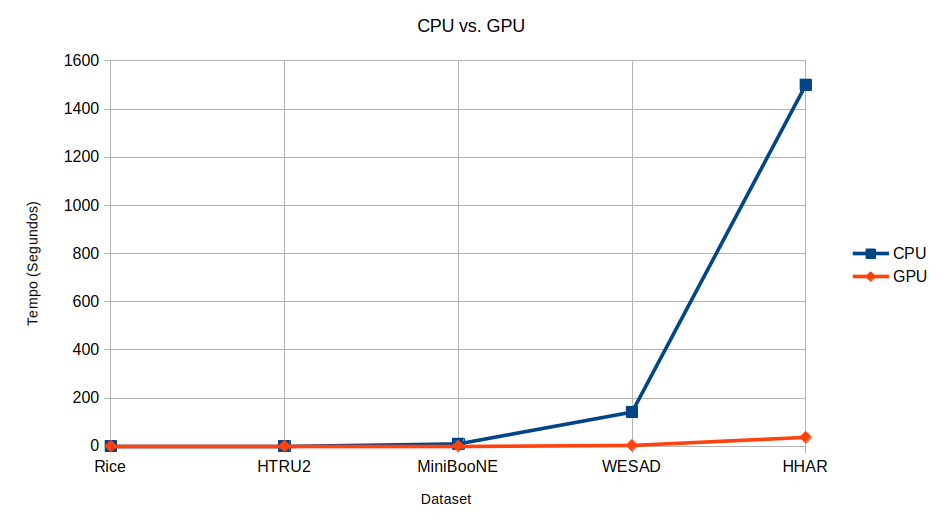
\includegraphics[width=0.95\textwidth]{kMeansAvgTime.png}
  \label{fig:kMeansAvgTime}
\end{figure}

\textbf{TODO: Adicionar as informações em forma de tabela também.}

\begin{figure}[h]
  \caption{Ganho médio de velocidade do k-means}
  \centering
  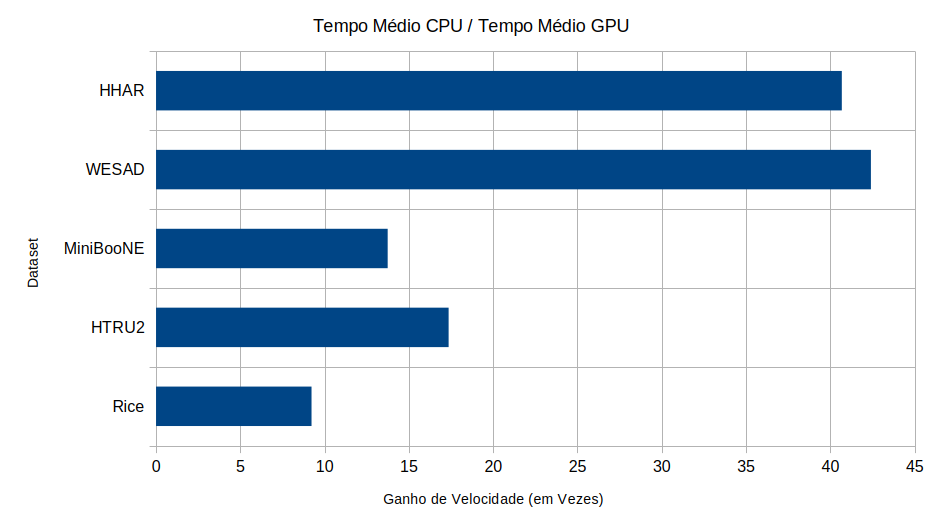
\includegraphics[width=0.95\textwidth]{kMeansAvgSpeedup.png}
  \label{fig:kMeansAvgSpeedup}
\end{figure}

% \begin{figure}[h]
%   \caption{Figura \ref{fig:kMeansAvg}, com zoom nos primeiros três menores datasets}
%   \centering
%   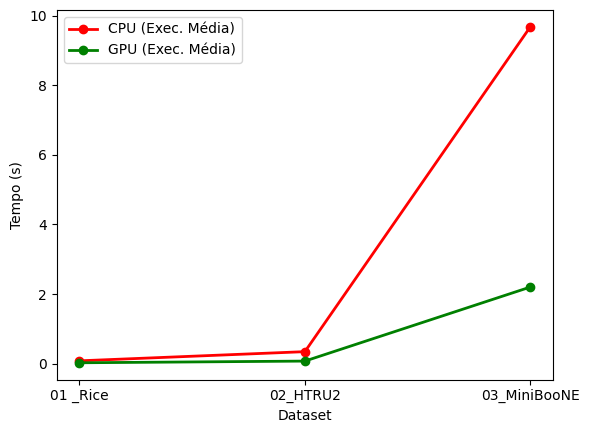
\includegraphics[width=0.95\textwidth]{kMeansResultsAvgZoomed.png}
%   \label{fig:kMeansAvgZoomed}
% \end{figure}



% * ####################################

\section{Precisão}
\label{sec:testesDePrecisao}

% TODO
% TODO
% TODO: Vide abaixo
% TODO
% TODO

\textbf{TODO: Escrever uma seção apresentando e discutindo os resultados dos testes de precisão e corretude rodados com cada dataset e implementação do k-means.}





% * ############################################################################

\chapter{Conclusões e Trabalhos Futuros}

% TODO
% TODO
% TODO: Vide abaixo
% TODO
% TODO

\textbf{TODO: Escrever capítulo com conclusões do trabalho + sugestões do que prosseguir para trabalhos futuros.}





% * ############################################################################





% * ############################################################################
% * ELEMENTOS PÓS-TEXTUAIS
% * ############################################################################

\postextual


% * ############################################################################
% * Referências bibliográficas
% * ############################################################################

\bibliography{references}


% * ############################################################################
% * Apêndices TCC: só mantenha se for pertinente.
% * ############################################################################

% ##################
% Inicializando os apêndices
% ##################

% \begin{apendicesenv}
  
% % Imprime uma página indicando o início dos apêndices
% \part[apendices]{Apêndices}

% * ############################################################################
% \chapter{Quisque libero justo}
% * ############################################################################

% \lipsum[50]

% * ############################################################################
% \chapter{Coisas que fiz e que achei interessante mas não tanto para entrar no corpo do texto}
% * ############################################################################

% \lipsum[55-57]

% \end{apendicesenv}


% * ############################################################################
% * Anexos (so mantenha se pertinente)
% * ############################################################################

% ##################
% Inicia os anexos
% ##################

\begin{anexosenv}

% Imprime uma página indicando o início dos anexos

\part[anexos]{Anexos}





% * ############################################################################
\chapter{Eu sempre quis aprender latim}
% * ############################################################################

\lipsum[30]





% * ############################################################################
\chapter{Coisas que eu não fiz mas que achei interessante o suficiente para colocar aqui}
% * ############################################################################

\lipsum[31]





% * ############################################################################
\chapter{Fusce facilisis lacinia dui}
% * ############################################################################

\lipsum[32]





% ##################
% Finalizando anexos
% ##################

\end{anexosenv}





% * ############################################################################
% * Índice Remissivo
% * ############################################################################

\printindex





% * ############################################################################

\end{document}
